%!TEX root = ../swiatlow_thesis.tex
\label{chapter:jets-and-substructure}
\section{The Goal of Jets}

The goal of particle physics experiments--- as Chapter~\ref{chapter:detector} will describe--- is to measure the outgoing particles produced in collisions in order to reconstruct the short lived intermediate states which describe the fundamental processes of nature. Final state particles such as electrons and muons and photons are measured through their interactions with a detector, and their 4-vectors are used to reconstruct the event and the interesting particles produced in the collision. 

Sections~\ref{chapter:sm:qcd:freedom} and \ref{chapter:sm:qcd:confinement} seem to throw a wrench into this program: quarks and gluons, two types of commonly produced particles, cannot be measured directly because of their interactions with the Strong Nuclear Force and the process of \textit{confinement}. Confinement is the process which hides color charge from the world: colored particles always form color neutral pairs and triplets, and in the process create a shower of associated color neutral particles. Thus what interacts with a detector is not just one particle, like in the case of an electron or a muon, but instead a large spray of hadrons which originate from the original parton.

Is it possible to reconstruct the 4-vectors of quarks and gluons? What information is lost in the showering process? Can the showering process itself tell us something about the physics of the collision? The answer to these questions is what we look for when we study \textit{jets}. This is the whimsical, though certainly appropriate, name for the collimated sprays of particles produced by quarks and gluons as they shower and hadronize. 

Because strongly interacting particles are so commonly produced in LHC collisions, understanding jets is integral to being able to reconstruct events. This chapter addresses the theoretical issues of jet reconstruction, describing first how 4-vectors corresponding to QCD partons are constructed and then describing some aspects of the emerging field of \textit{jet substructure}, in which the shapes and structur of jets can be used to infer new information about events.



\section{Jet Algorithms}

At first glance, the process of jet identification should be trivial. Figure~\ref{fig:jets:dijet}, for example, has two clearly identified showers of particles on either side of the detector: we can easily identify these groupings by eye, sum up 4-momenta of the calorimeter cells therein, and then analyze our di-jet event.


%%%%%%%%%%%%%%%%

\begin{figure}
\centering
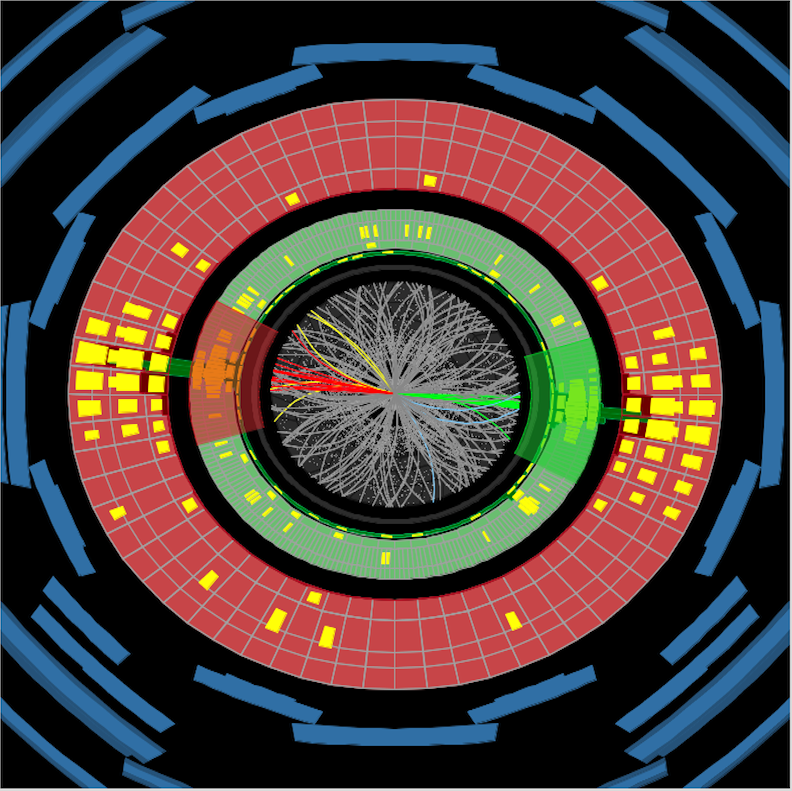
\includegraphics[width=0.7\textwidth]{dijet.png}
\label{fig:jets:dijet}
\caption{An example dijet event recorded in the ATLAS detector.}
\end{figure}

%%%%%%%%%%%%%%%% 

But what happens when events become more complicated? How many jets are there in Figure~\ref{fig:jets:4-jet}? Or in the event displays in Figure~\ref{fig:jets:many-jet}? As the complexity of the event increases, it becomes increasingly difficult to tell the differences between jets simply by eye. Moreover, while this kind of ad-hoc identification is possible when discussing handfuls of events, the LHC detectors record 500 events per second, or even more, so our by-eye approach is not going to scale to the task at hand. 

%%%%%%%%%%%%%%%%

\begin{figure}
\centering
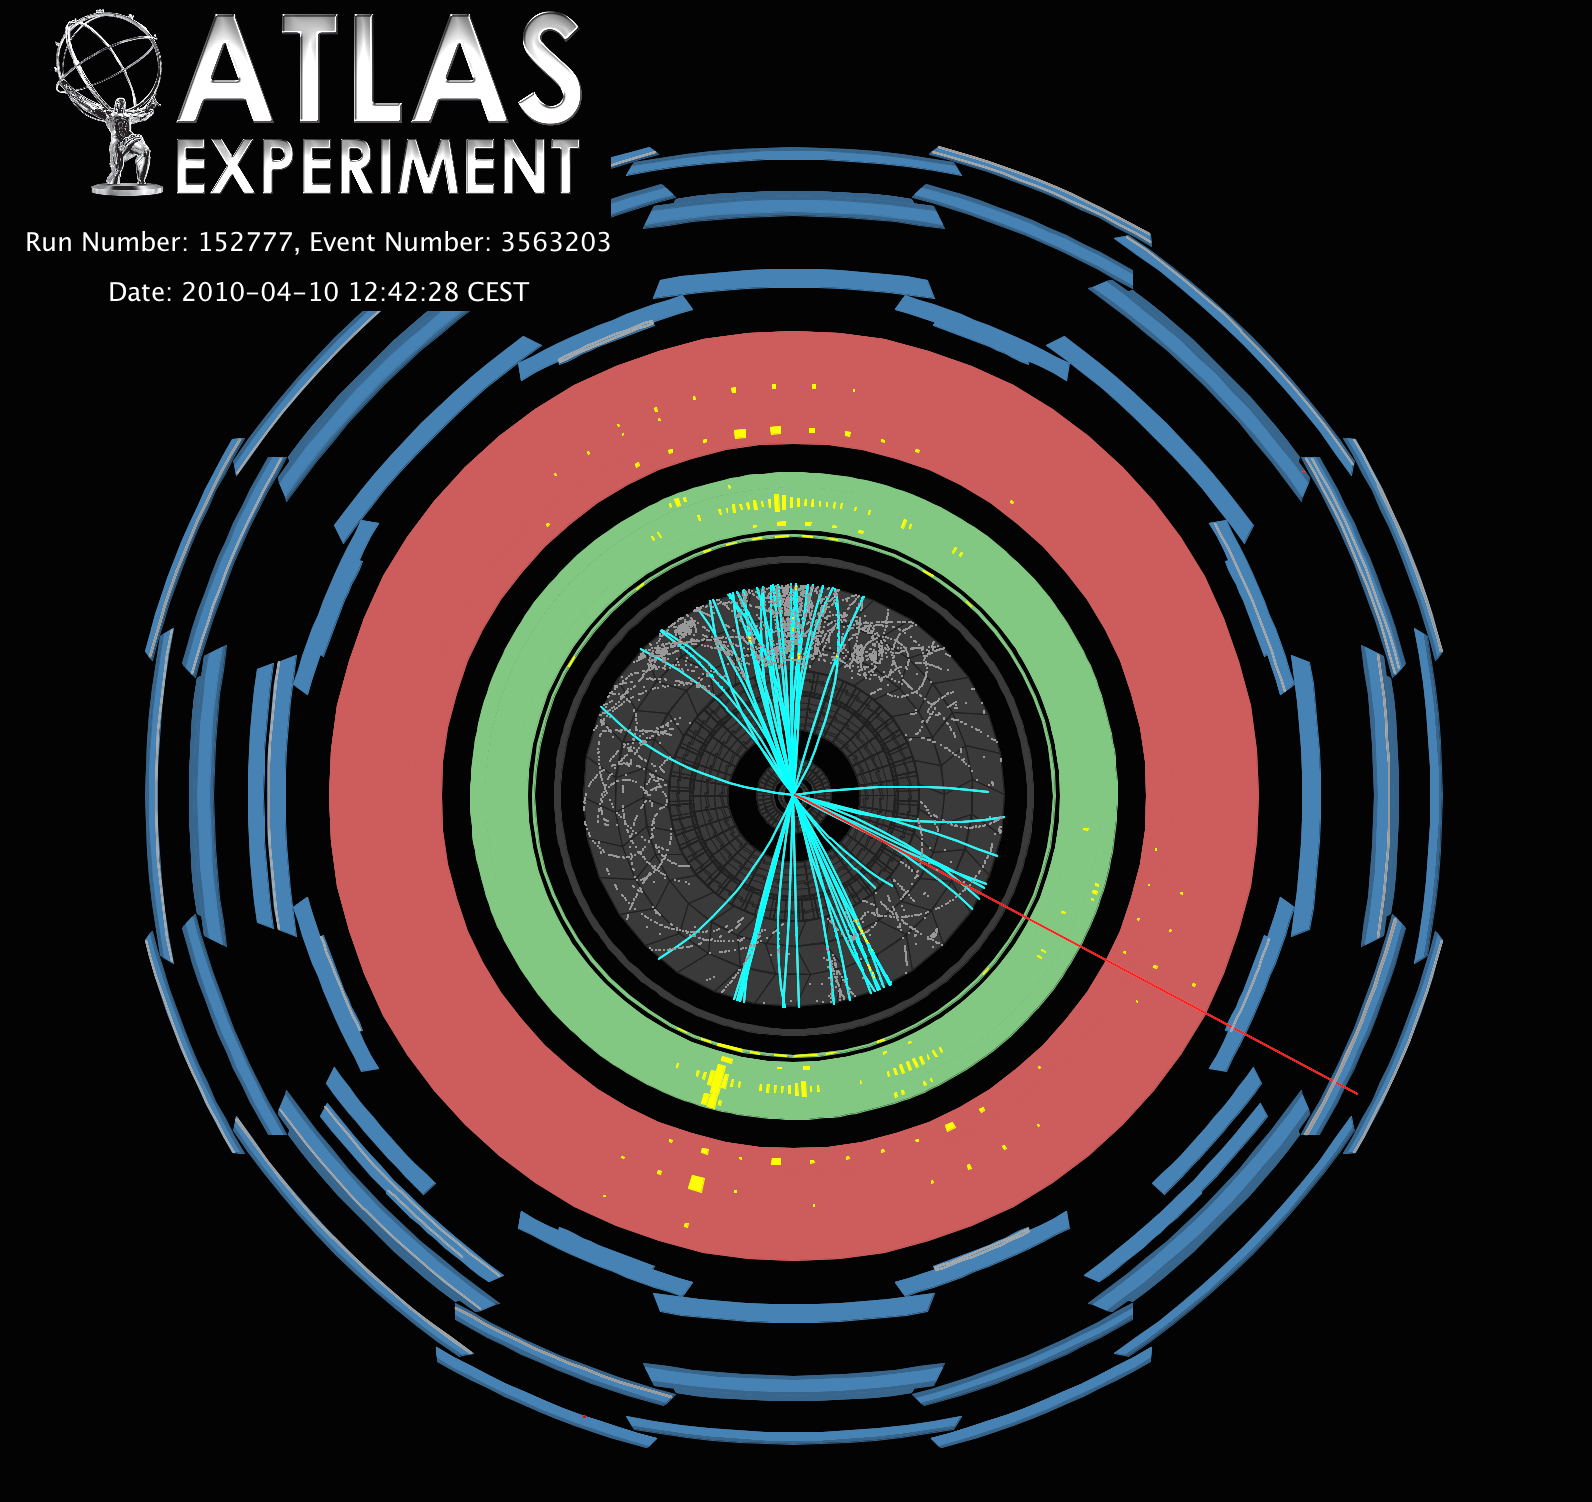
\includegraphics[width=0.7\textwidth]{4-jet.png}
\label{fig:jets:4-jet}
\caption{An example 4-jet event recorded in the ATLAS detector.}
\end{figure}

%%%%%%%%%%%%%%%% 


%%%%%%%%%%%%%%%%

\begin{figure}
\centering
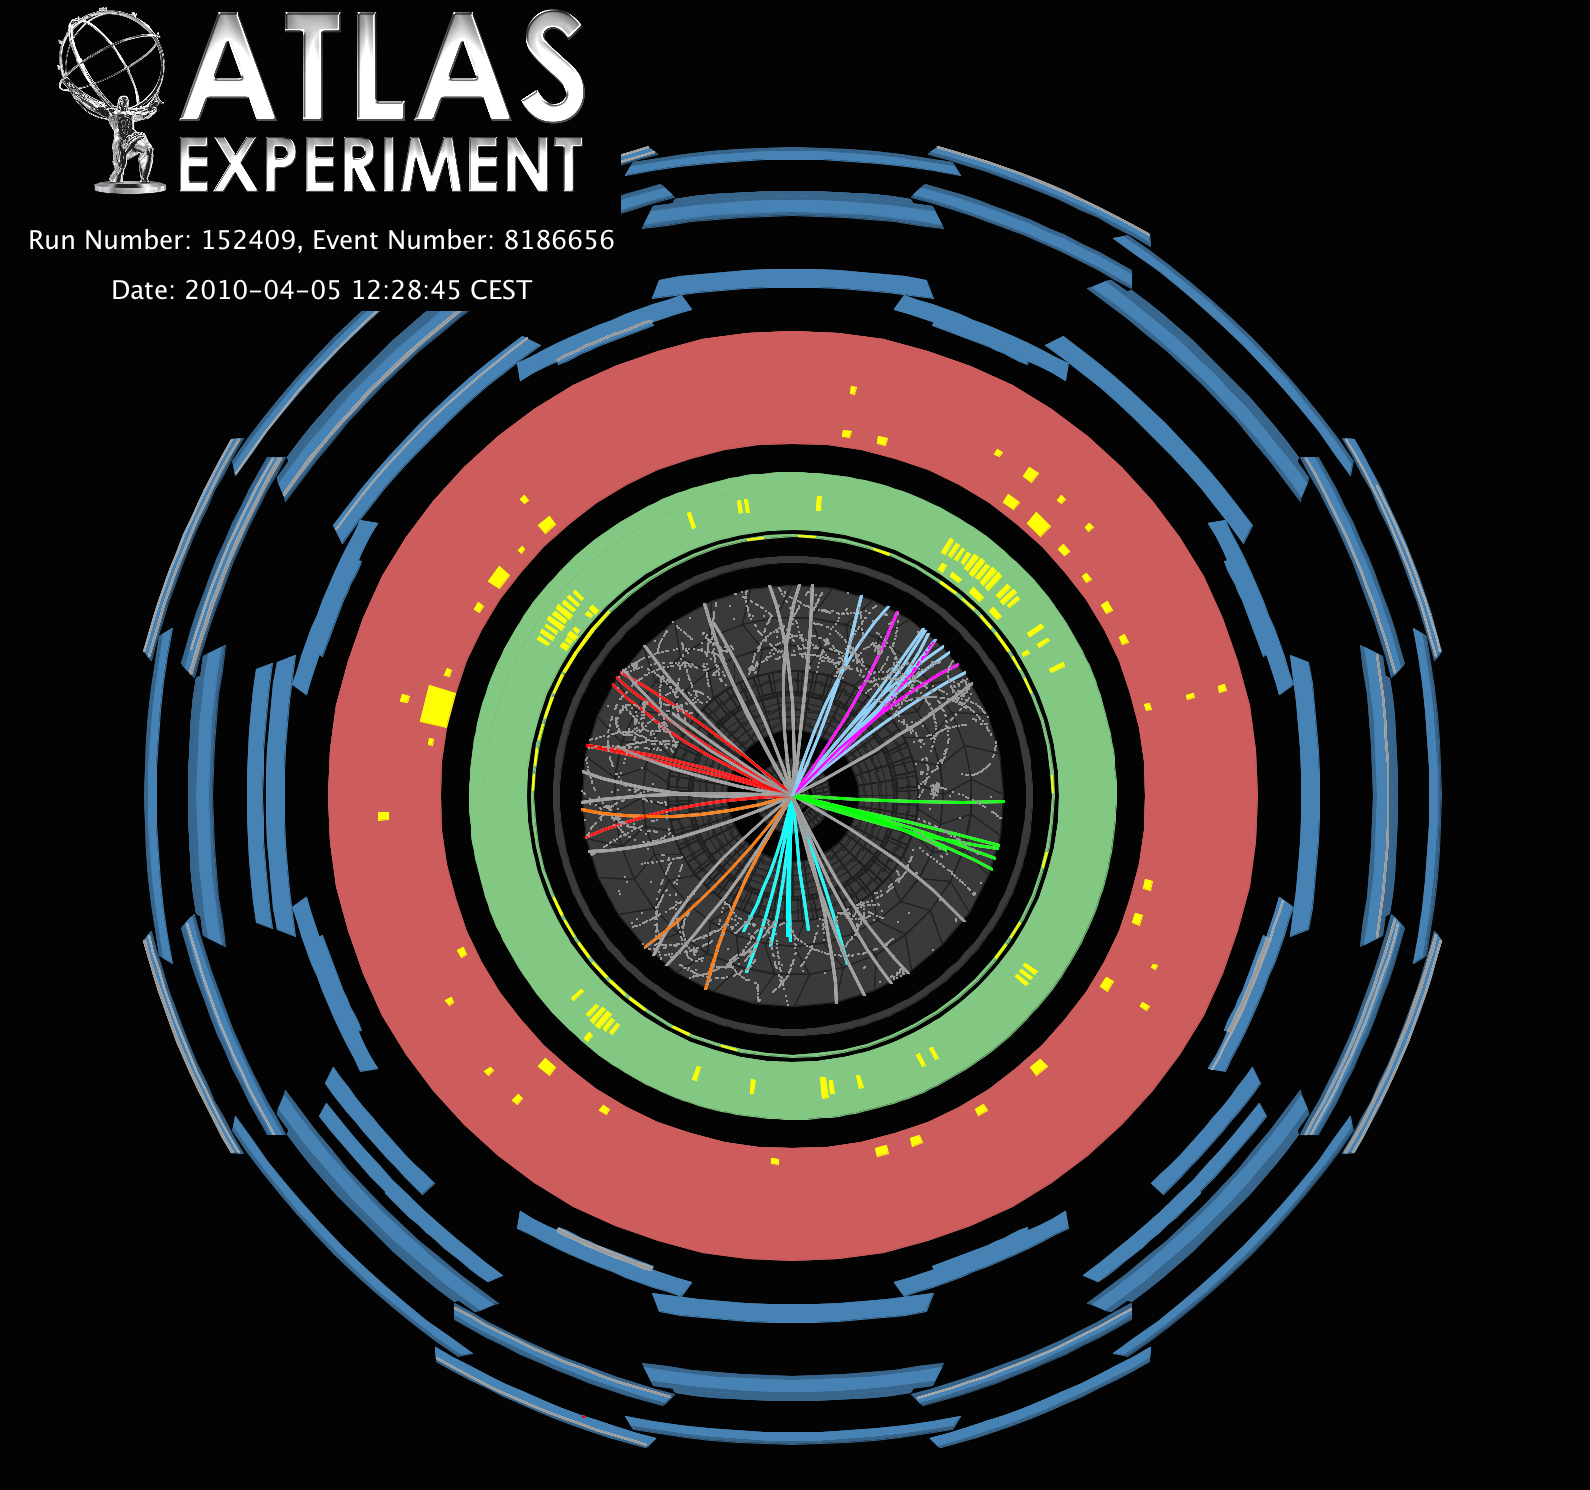
\includegraphics[width=0.45\textwidth]{6-jet.png}
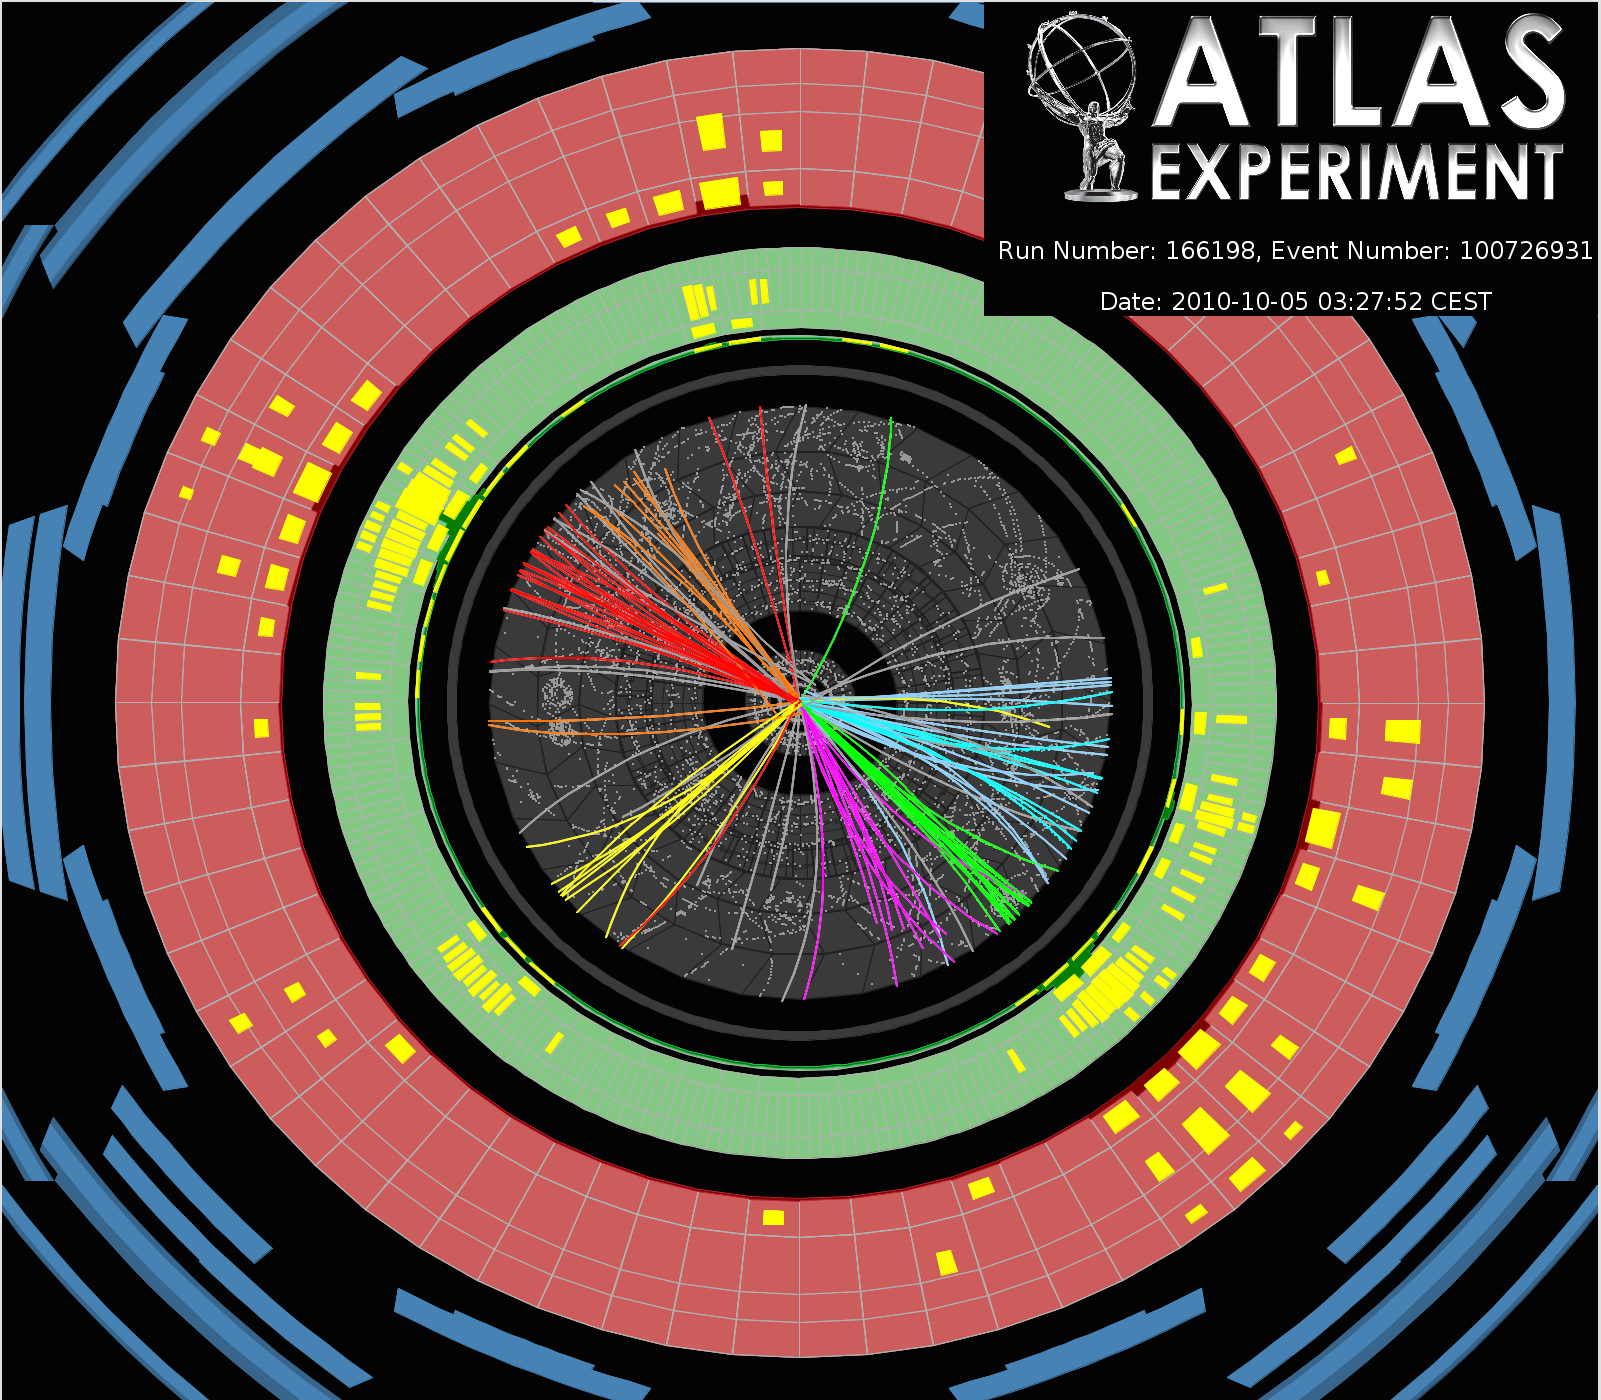
\includegraphics[width=0.45\textwidth]{8-jet.png}
\label{fig:jets:many-jet}
\caption{An example 6- and 8-jet event recorded in the ATLAS detector: as the complexity of events increases, the difficulty of cleanly identifying jets becomes more difficult.}
\end{figure}

%%%%%%%%%%%%%%%% 


The introduction of \textit{jet algorithms} solves this problem~\cite{Jetography}. Jet algorithms provide a detailed prescription for how to combine different detector objects (or simulation-level particles) into jets, and are used to automate the process of jet finding over the billions of events that the colliders produce.

What features connect or distinguish jet algorithms? A simple example is how they handle one completely isolated particle: any reasonable algorithm should identify that one particle as a jet. But what about two close-by particles, in the case, for example, that a quark radiated a gluon? Usually the algorithm has some distance parameter, typically denoted $R$, which specifies a distance scale over which particles should be combined or not. One other question is how these two particles are combined: should their 4-vectors be added, or just their energies, etc? The combination of the jet algorithm, the distance parameter, and the recombination scheme specify a \textit{jet definition}\cite{Jetography}. A jet algorithm should be able to run on a parton-level event from simulation, a hadron-level event from simulation after a power shower and hadronization, or on detector level objects (calorimeter energy measurements, tracks, etc). In all cases the algorithm takes in 4-vectors and returns 4-vectors.

What does it mean to be a ``good'' jet algorithm? This question has been at the heart of hadronic analyses for decades, but historically there was often little agreement on what metrics should be used to evaluate algorithms, with an especially large disconnect between the needs of theorists (focused on calculability) and experimentalists (focused on speed and ease of use). The Snowmass Accords of 1990 was the first effort to define a set of criteria jet algorithms should try to achieve~\cite{Huth}:
%
\begin{itemize}
\item Simple to implement in an experimental analysis;
\item Simple to implement in the theoretical calculation;
\item Defined at any order of perturbation theory;
\item Yields finite cross section at any order of perturbation theory;
\item Yields a cross section that is relatively insensitive to hadronization
\end{itemize}
%
In practice, it took twenty years for experiments to adopt something compatible.

\subsection{Cone Algorithms} 

In the meantime, experiments tended to use a class of algorithms referred to as \textit{cone algorithms}~\cite{Jetography}. Typically, the algorithms would follow the general steps of:
%
\begin{enumerate}
\item Find a seed, typically the highest energy object
\item Draw a cone of size $R = \sqrt{\Delta \eta^2 + \Delta \phi^2}$ around the cluster: join all objects inside the cone with the seed
\item Remove this object: it is a finished jet
\item Proceed with the next highest seed, returning to step 1
\item When all seeds are used up, run a secondary split/merge step on closeby jets to resolve ambiguities
\end{enumerate}
%
Improvements such as the iterative cone,  overlapping cone, or midpoint cone algorithms modify the details, usually by adding additional refinement stages, where the center of the jet is allowed to drift away from the seed.

The main advantage of the cone algorithms was their speed: determining jets was simply a matter of computing distances to the seed, and so scaled as $O(N)$ with the number of objects to be clustered, and so certainly the first point of the Snowmass Accord was fulfilled. Unfortunately, cone algorithms have a much more difficult time with the remaining points.

\subsection{IRC Safety}

The last four parts of the Snowmass Accords detail the robustness of a jet clustering algorithm: how sensitive is the clustering to various fluctuations, and how reliable is it when used to make theory calculations and predictions? The assessment of these issues, somewhat poorly defined by Snowmass but much better understood now, lies in the definitions of \textit{infrared} and \textit{colinear} safety, often referred to together as IRC safety~\cite{Jetography}. Infrared safety is the guarantee that the result of a jet algorithm does not change if there is additional very soft radiation in the event. A low energy gluon emission is possible at any point in the showering of a jet, but is such a small effect that the algorithm--- which is trying to tell us about the initiating parton--- should not be affected by it. Colinear safety, on the other hand, is the guarantee that if a one hard particle were to split into two nearly colinear softer particles, that the algorithm would return a consistent result. Once again, the exact evolution of the parton shower should not matter: the same energy is heading in more or less the same direction, and our algorithm should be robust to the number of particles this energy comes in.

%%%%%%%%%%%%%%%%

\begin{figure}
\centering
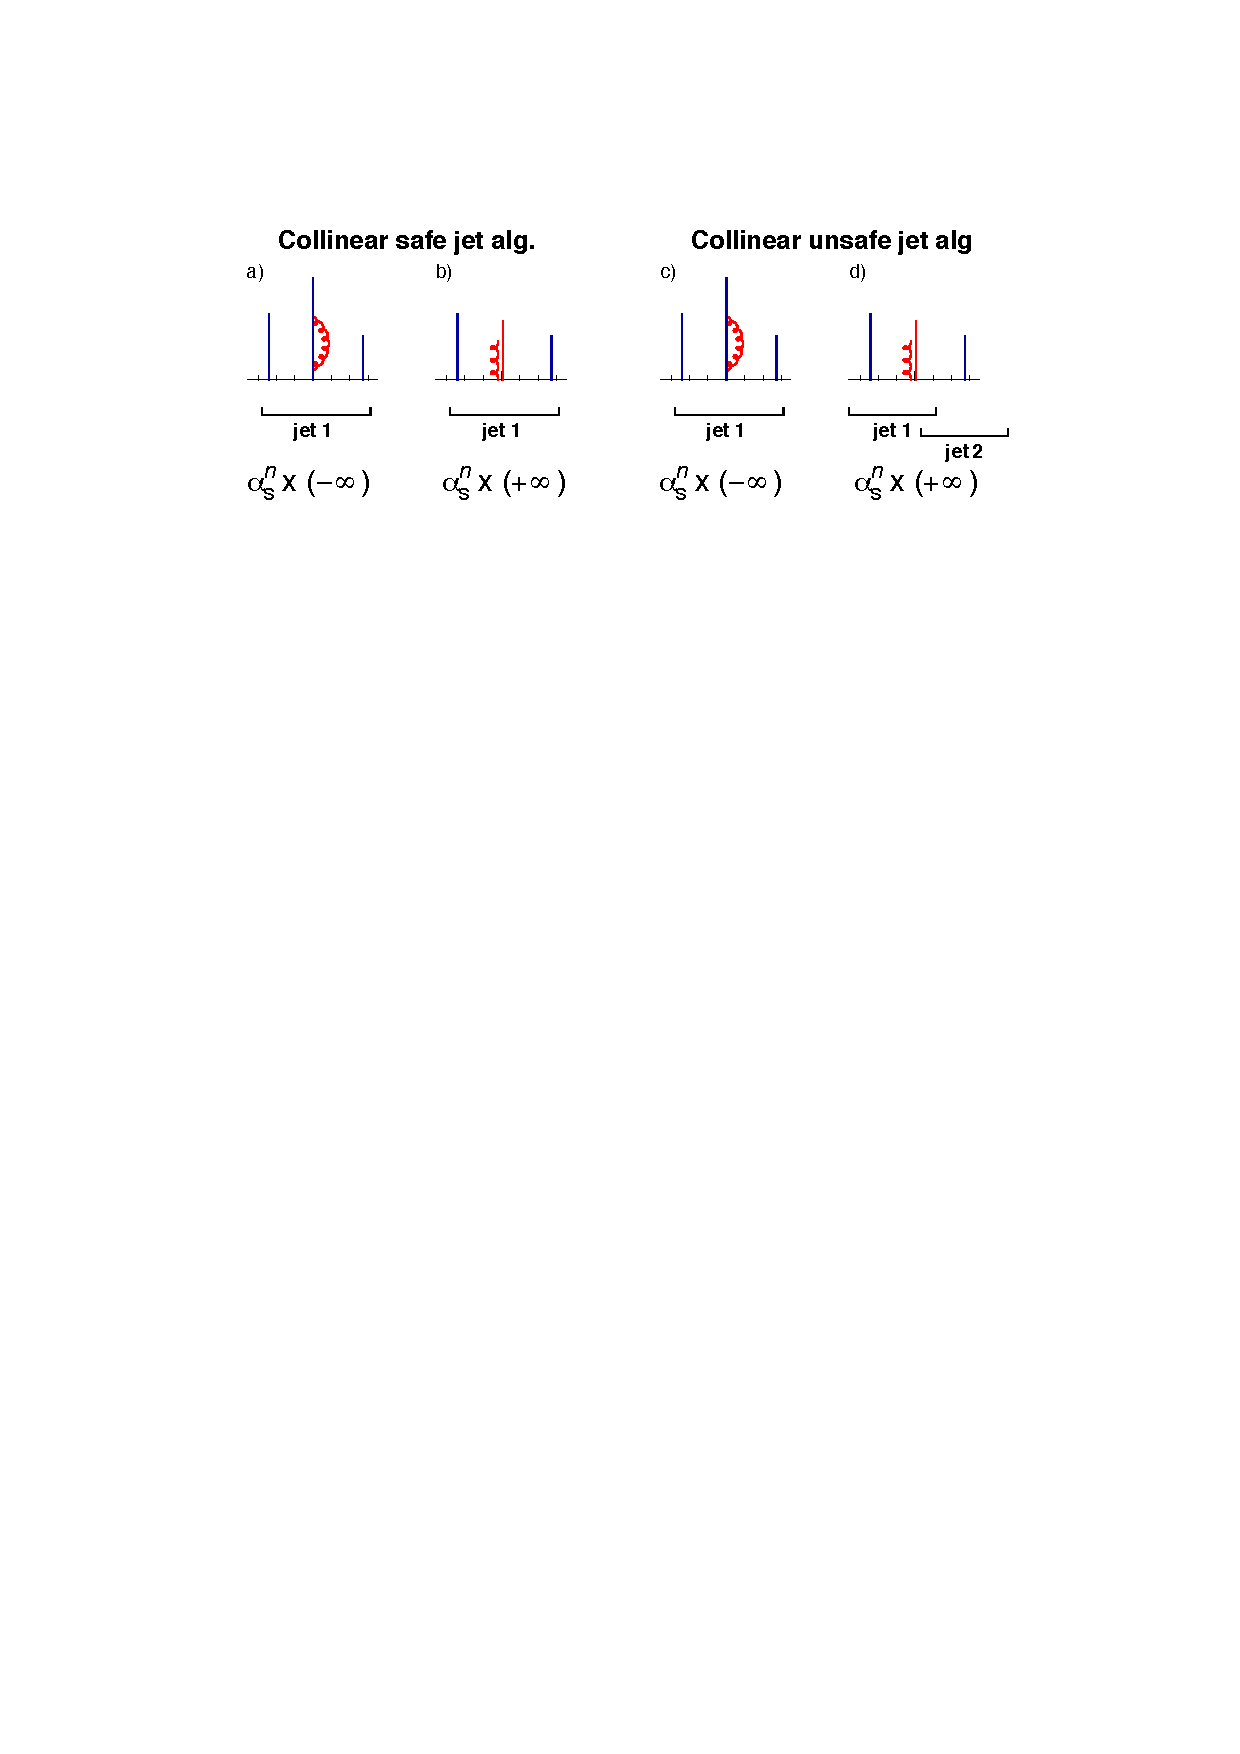
\includegraphics[width=0.7\textwidth]{ir.pdf}
\label{fig:jets:ir}
\caption{An example of a colinear splitting which changes the result of a jet algorithm. The $x$-axis indicates angular position; the $y$-axis indicates the energy of a particle. Configurations a, b, c, d all have the same total energy, but while b creates one jet, d creates two. Figure from \cite{Jetography}.}
\end{figure}

%%%%%%%%%%%%%%%% 

%%%%%%%%%%%%%%%%

\begin{figure}
\centering
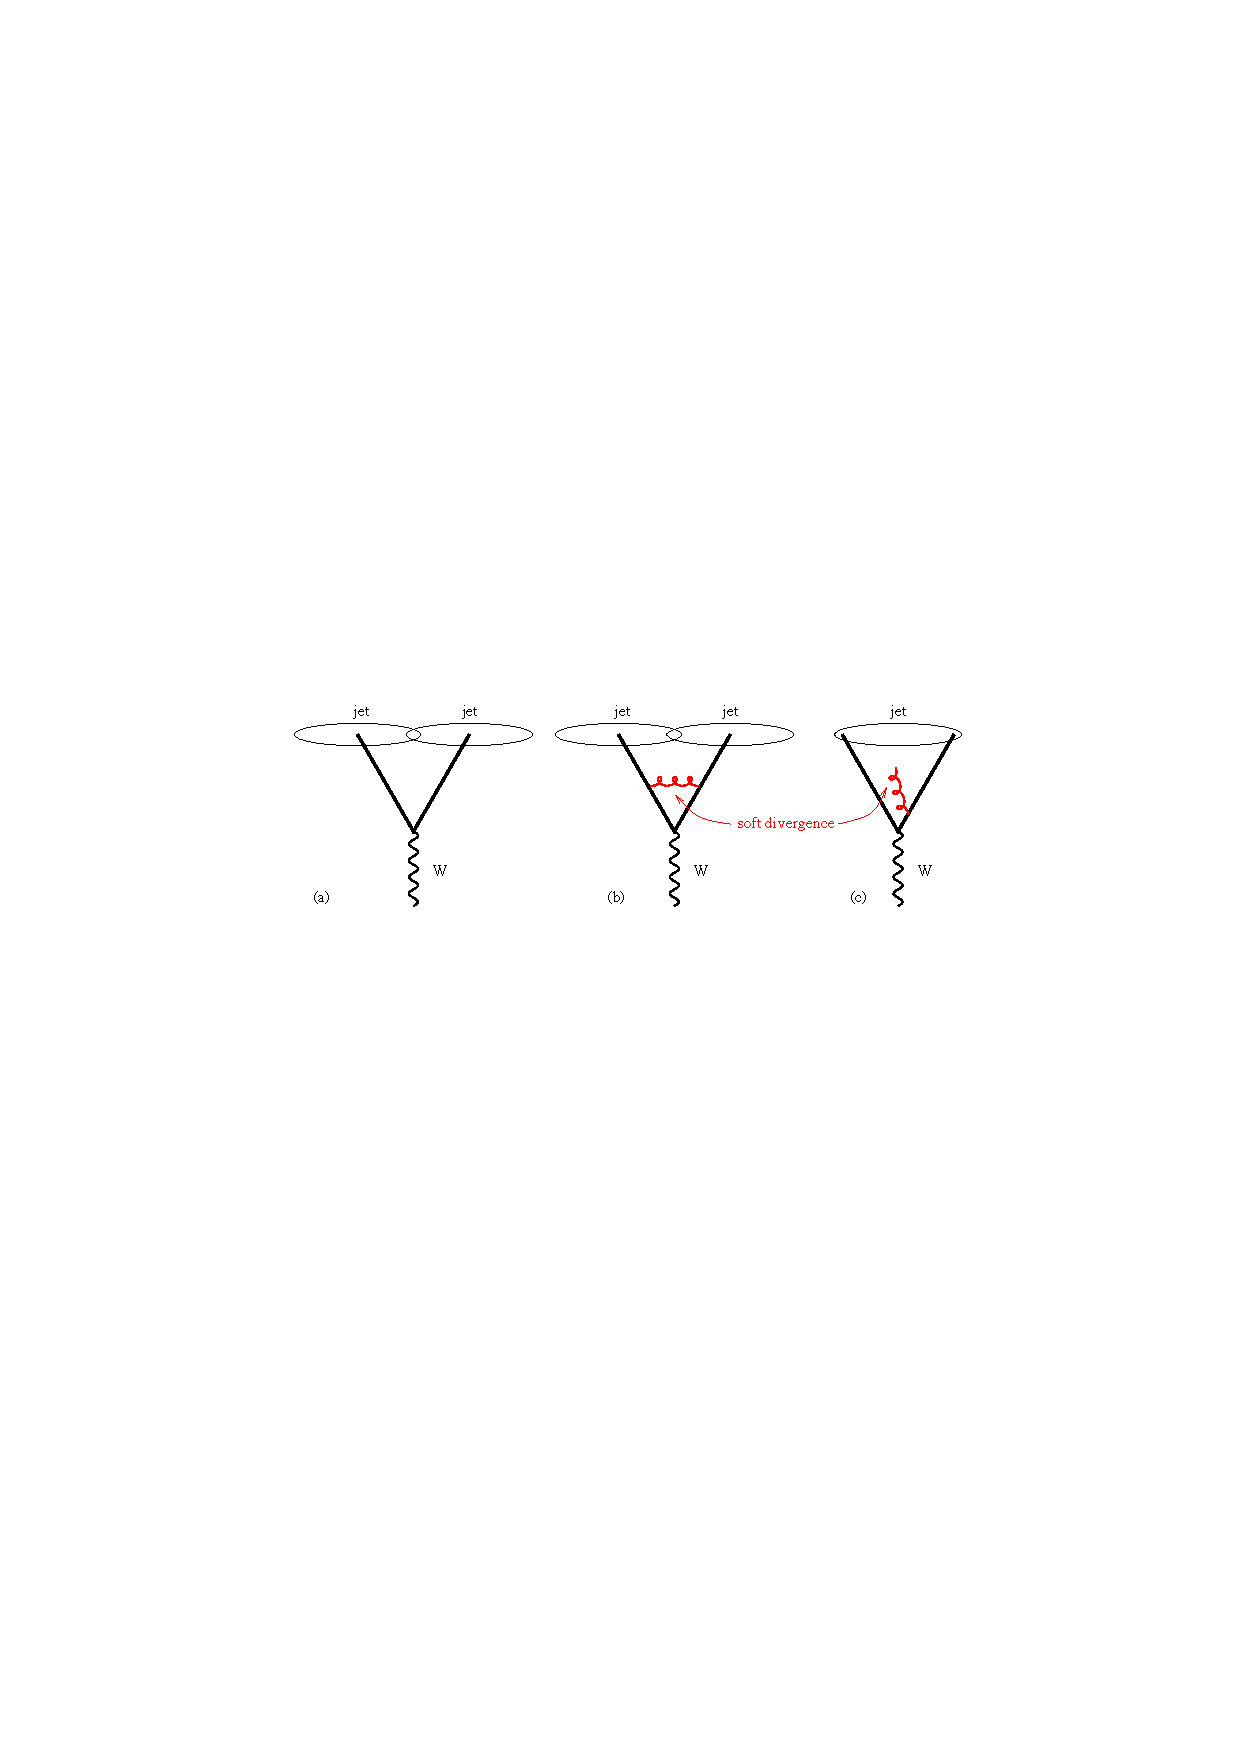
\includegraphics[width=0.7\textwidth]{c.pdf}
\label{fig:jets:c}
\caption{An example of an infrared (i.e. very soft) emission which changes the result of a jet algorithm. In this case, a softly emitted gluon in c causes extra radiation which creates an extra seed between the two separated jets of a and b; this extra seed can, in some iterative cone algorithms, cause the merging of these two jets. Figure from \cite{Jetography}.}
\end{figure}

%%%%%%%%%%%%%%%% 

The weakness of cone algorithms to colinear effects is easiest to understand: all cone algorithms use seeds of various sorts, and the splitting of one hard particle can cause the two softer particles to be separately measured, and therefore fall under threshold. This is demonstrated schematically in Figure~\ref{fig:jets:ir}, where particle configuration d results in two jets in the collinear unsafe algorithm, even though the distribution of energy is nearly identical to that of configuration a.

Infrared safety is a more subtle effect, and depends on the details of the cone algorithm's iteration or split-merging steps. For example, in Figure~\ref{fig:jets:c}, the extra soft emmission between two otherwise well separated jets can cause a new soft seed to appear between the jets: the merging step of many cone algorithms looks precisely for additional radiation between jets to decide if a pair should be merged, and this can cause the number of jets in the event to change.

What, exactly, are the consequences for failing to respect these requirements? The obvious pitfall is sensitivity to the exact development of the parton shower, which point 5 of the Snowmass Accords also requires us to avoid. IRC safety is also closely related to the middle three points of the Snowmass Accords, which all deal with calculations of jet properties (cross-sections, \pt spectra, and so on). In particular, soft emmissions and colinear splittings (the IR and the C) in perturbative calculations are actually divergent and therefore blow up the calculation. The saving grace of the calculation is that these terms come in with opposite signs, and therefore cancel--- but if the jet algorithm separates these infinities into separate objects, they will not properly cancel~\cite{Jetography}. For these reasons, both non-perturbative parton shower simulations and perturbative theoretical calculations are automatically of limited use in comparisons to data: if we want to test our understanding of QCD in various regimes, we need jet algorithms which respect these sensitivities.

Note that the process of measuring an event always softens the effects of IRC unsafety: limited angular resolution can mean that a colinear split is measured together still, or measurement thresholds can prevent infrared radiation from occuring and spoiling the merging process. All of these effects are by definition very detector specific, however: the robustness of a theoretical calculation should not have to depend on the angular size of the readout of a calorimeter.

What exactly cause this sickness of the cone algorithms? The main issues are at the start and at the end of the clustering: the seed and the split/merge process. If we can remove seeds from the process, we can prevent the colinear safety issues; if we define the algorithm without drawing an explicit cone, we can remove much of the ambiguities that require the split/merging step.

\subsection{Sequential Recombination Algorithms}
\label{chapter:jets-and-substructure:sequential}


Sequential recombination algorithms do exactly both of these things. The idea behind them is to focus not on seeds and the cone around them, but instead on the relationships between closeby particles. In particular, there is always a \textit{distance metric} between pairs of particles, and in every iteration of the algorithm, the pair with the minimum distance is \textit{combined} if their distance is below some threshold. The process continues until no more merges are possible~\cite{Jetography}.

This strategy clearly improves the situation with seeds: there is never an energy dependent ``primary'' particle used to create a jet. The distance metrics can be weighted by energy themselves to ensure that jets follow energy flow throughout the event, but the iterative merging process removes the pathological dependencies on single particles which plagued cone algorithms. The merging process also has a clear stopping point defined: this lets the boundaries of jets grow naturally, without the concerns of overlaps that a simple cone drawing adds.

%origins

The first sequential algorithms we used in $e^+/e^-$ collisions: these were natural targets, as the ``clean'' leptonic collisions do not produce the additional underlying event contamination and large jet multiplicity inherent to hadronic collisions. Particle multiplicity is always a concern when analyzing events with sequential recombination algorithms, as the minimized distance calculation typically goes as $O(N^3)$ and can become prohibitively expensive at hadron colliders~\cite{Jetography}\footnote{Indeed, at LEP collisions on the $Z$ peak, typically 40 particles were produced--- while 4000 are expected at LHC 14 TeV collisions!}. The first successful application at an $e^+/e^-$ machine was at JADE, and used a distance metric:
%
\begin{equation}
y_{ij} = \frac{2 E_i E_j (1 - \cos \theta_ij)}{Q^2}
\end{equation}
%
where $E$ are the particle energies, $\theta$ is the angle between particles, and $Q$ is the total energy of the event\cite{Jetography}. For massless particles, is just the invariant mass between a pair: the algorithm proceeds to merge objects that have the smallest masses. Jets are merged if $y_\mathrm{min} < y_\mathrm{cut}$, the jet resolution threshold: the number of jets is clearly dependent on the value of this parameter, with more jets produced with a smaller $y_\mathrm{cut}$.

The IRC safety of the JADE algorithm is clear. Soft particles (the worry of infrared safety) are merged together quickly as they have small energies, and colinear particles are merged quickly because of their small angular splitting. The JADE algorithm has a particularly interesting pathology in that soft particles on the opposite sides of the detector can be clustered together if they each have a very small energy: this clearly goes against our intuition that jets should be local groupings, and so improvements became necessary.

The $k_t$ algorithm was the solution--- the only difference is to replace the distance metric with
%
\begin{equation}
y_{ij} = \frac{2 \min(E_i^2,E_j^2) (1-\cos{\theta_{ij}})}{Q^2}.
\end{equation}
%
Considering only the minimum energy of two particles guaranteed that close-by particles would be preferred for matching over distant pairs, while preserving the IRC safety of the algorithm. This form is motivated strongly also by the probability of colinear splittings in QCD from one parton $k$ to a pair $ij$ (in the limit of soft $i$ or $j$), which generally go as:
%
\begin{equation}
\frac{P_{k\rightarrow ij}}{dE_i d\theta_{ij}} \approx \frac{\alpha_s}{\min(E_i E_j) \theta_{ij}}.
\end{equation}
%
These features made the \kt algorithm a favorite of the LEP experiments~\cite{Jetography}.

Several assumptions go into this algorithm which preclude its use at a hadron collider. The main difficulty in applying it is the assumption of a full measurement of the energy of the event, whereas the varying longitudinal boosts at a hadron collider (because of the unknown, and possibly unbalanced momentum fractions of the incoming partons) mean that only transverse energy is generally meaningful (as this quantity is invariant under longitudinal boosts). Therefore, the following terms are defined for use of the \kt family at hadron colliders:
%
\begin{align}
d_{ij} &= \min(p_{Ti}^{2p}, p_{Tj}^{2}) \frac{\Delta R_{ij}^2}{R^2} \nonumber\\
\Delta R^2 &= (\phi_i - \phi_j)^2 + (y_i - y_j)^2\nonumber\\
d_{iB} &= p_{Ti}^{2p}
\end{align}
%
The algorithm proceeds almost identically to the $e^+/e^-$ version, but with a few small changes:
%
\begin{enumerate}
\item Find the minimum of all $d_{ij}$ and $d_{iB}$
\item If $d_{ij}$ is a minimum, combine the pair and return to 1; if $d_{iB}$ is a minimum, consider the particle a finished jet and remove it from the list, and then return to 1
\item Finish when there are no more particles.
\end{enumerate}
%
In this definition, $d_{ij}$ are once again the interparticle distances, and $\Delta R$ is an angular distance similar to $\theta_{ij}$ but which respects longitudinal boosts. $d_{iB}$ is the particle-beam distance: this corresponds to our understanding that most particles continue down the beampipe with no transverse momentum, and that clustering should come to an end when this set of particles is the closest to the $i$ in question. The former size parameter $y_\mathrm{cut}$ has been replaced by the distance parameter $R$: happily, $R$ has a bit more of a intuitive meaning, as it has the same units as the angular distance $\Delta R$. The last open parameter is $p$: for the \kt algorithm, $p=1$, but there are other options as well.
%modifications

Initial studies of the \kt algorithm at the D0 experiment at the Tevatron were somewhat dissappointing: they showed that not only was the clustering time was a major concern, but that the \textit{irregular shape} of the \kt jets led to sensitivity to the simulation of the underlying event. For many years these were convenient excuses for experimentalists to focus on the faster and more ``regular'' cone algorithms. The former concern was alleviated in 2006 when Gavin Salam and Matteo Cacciari released the seminal \texttt{FastJet} package, which used advances in computational geometry to reduce the complexity of \kt jet finding to $O(N \ln N)$--- faster than any other algorithm at the time~\cite{fj}. 

Concerns about jet shapes remained, however. Figure~\ref{fig:jets:kt} shows an example ATLAS simulated event with many final state quarks clustered with the \kt algorithm with $R=1.0$: the shapes of the jets are clearly quite different from the cone expectation. These shapes form from the clustering of soft particles to each other: as the softest particles are clustered first due to the structure of the distance metric, interesting shapes can arise because of the relative ease of a shower or the underlying event producing soft particles. A similar algorith, referred to as \CA, sets $p=0$ in the distance metric and therefore completely ignores the energy and uses only distances to match particles. Figure~\ref{fig:jets:ca} shows the same event display clustered with the \CA algorithm with $R=1.0$: the shape is quite similar to \kt, and features the same irregular pattern. Soft particles are likely to lie next to each other, and so the similarity should not be completely unexpected.  % and contain meaningful physics: if one imagines the QCD shower as a branching tree, then the soft particles consist of the furthest branchings.

%%%%%%%%%%%%%%%%

\begin{figure}
\centering
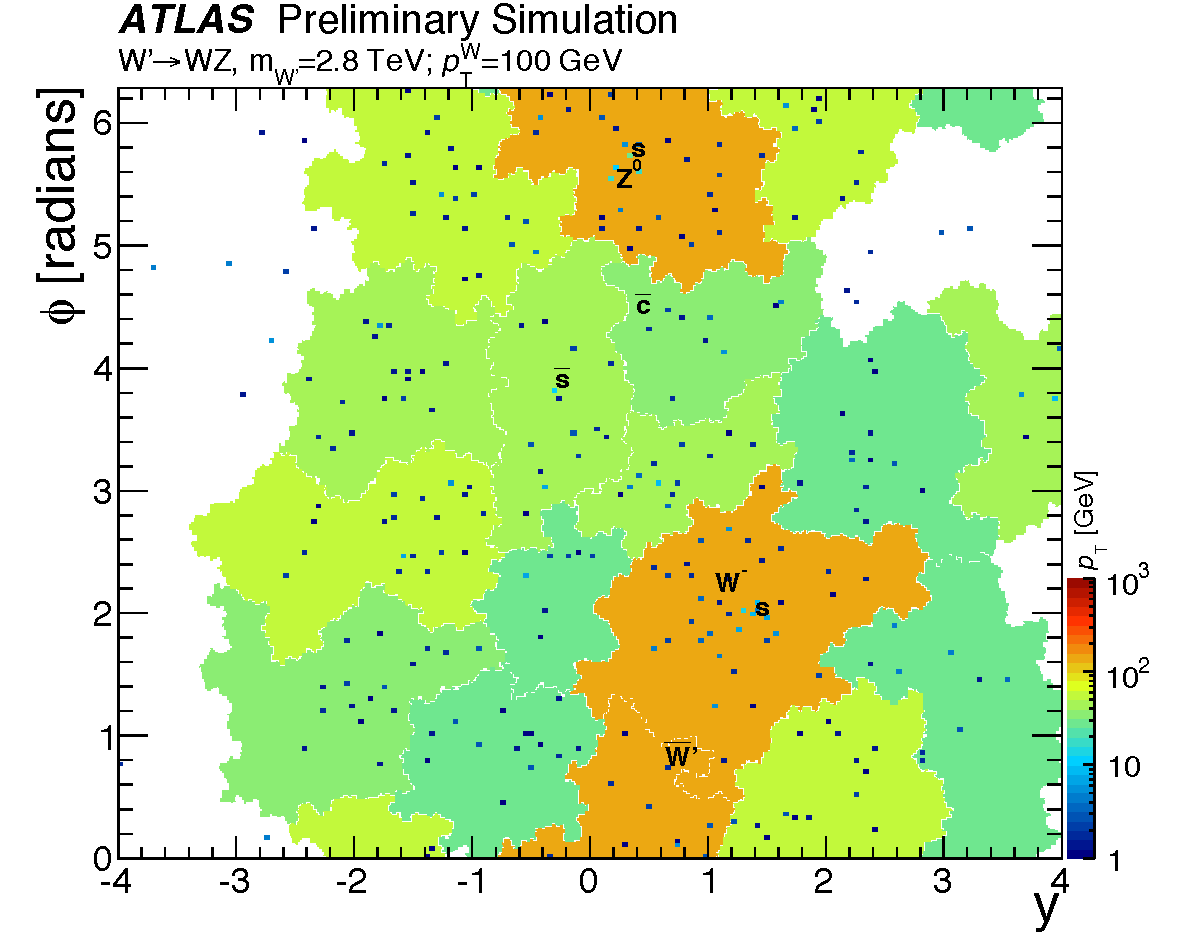
\includegraphics[width=0.7\textwidth]{kt.pdf}
\label{fig:jets:kt}
\caption{An example of a simulated ATLAS $W'\rightarrow WZ\rightarrow qqqq$ event, clustered with the \kt algorithm with $R=1.0$.}
\end{figure}

%%%%%%%%%%%%%%%% i

%%%%%%%%%%%%%%%%

\begin{figure}
\centering
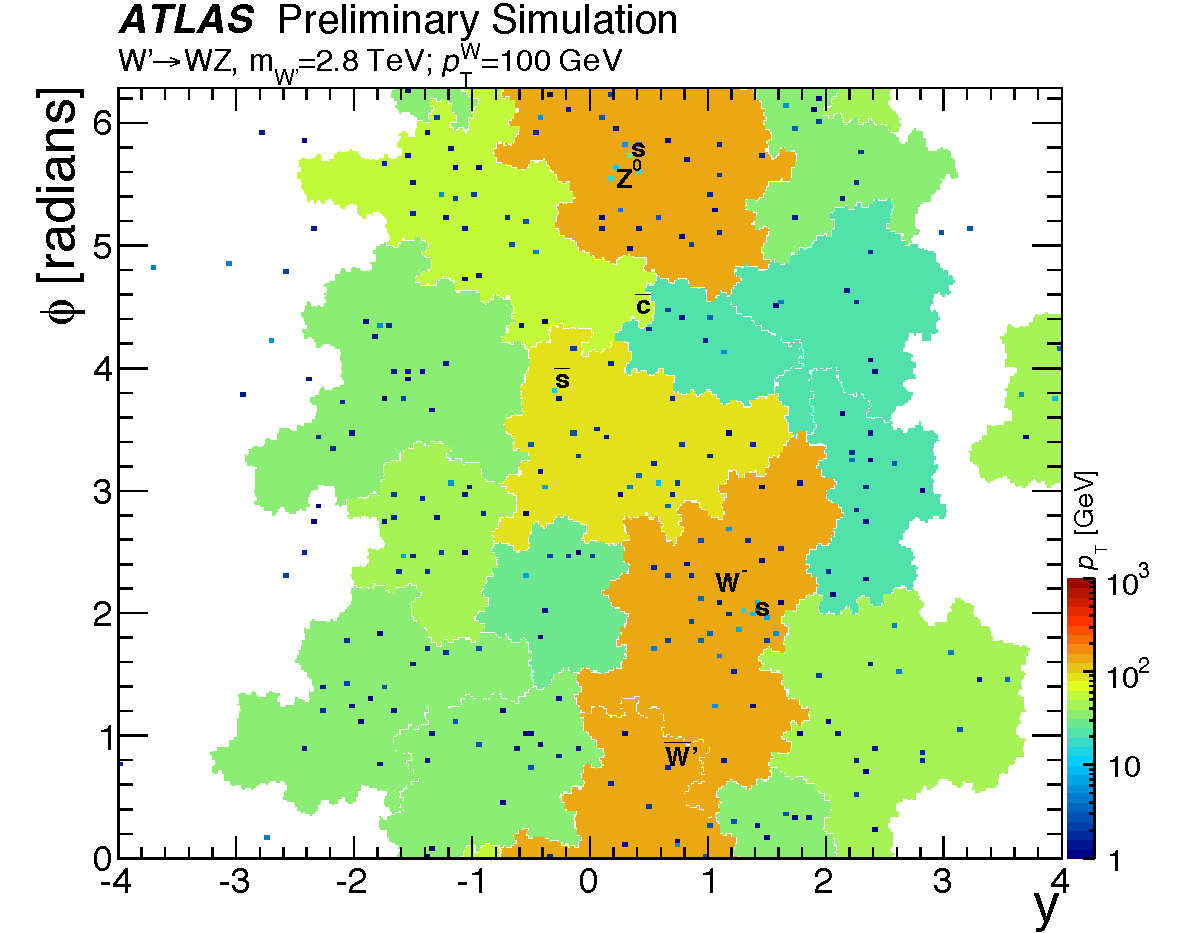
\includegraphics[width=0.7\textwidth]{ca.pdf}
\label{fig:jets:ca}
\caption{An example of a simulated ATLAS $W'\rightarrow WZ\rightarrow qqqq$ event, clustered with the \CA algorithm with $R=1.0$.}
\end{figure}

%%%%%%%%%%%%%%%% 




Are these shapes a problem? Theoretically, no--- they are well defined and IRC safe objects because of the structure of the algorithm that forms them. Experimentally, this was less clear--- was it possible to calibrate an object that whose shape was so sensitive to soft radiation? Concerns such as these motivated the introduction of the \antikt algorith, which sets $p=-1$ in the distance metric~\cite{Jetography}. Figure~\ref{fig:jets:akt} shows once again the same event, but clustered now with the \antikt algorithm with $R=1.0$. The structure is strikingly different: indeed, because the algorithm now preferentially clusters \textit{hard} particles first, the seed-like properties of cone algorithms are restored. However, because colinear particles are clustered first--- the $\Delta R$ term contributes to this--- IRC safety is still guaranteed~\cite{Jetography}.



%%%%%%%%%%%%%%%%

\begin{figure}
\centering
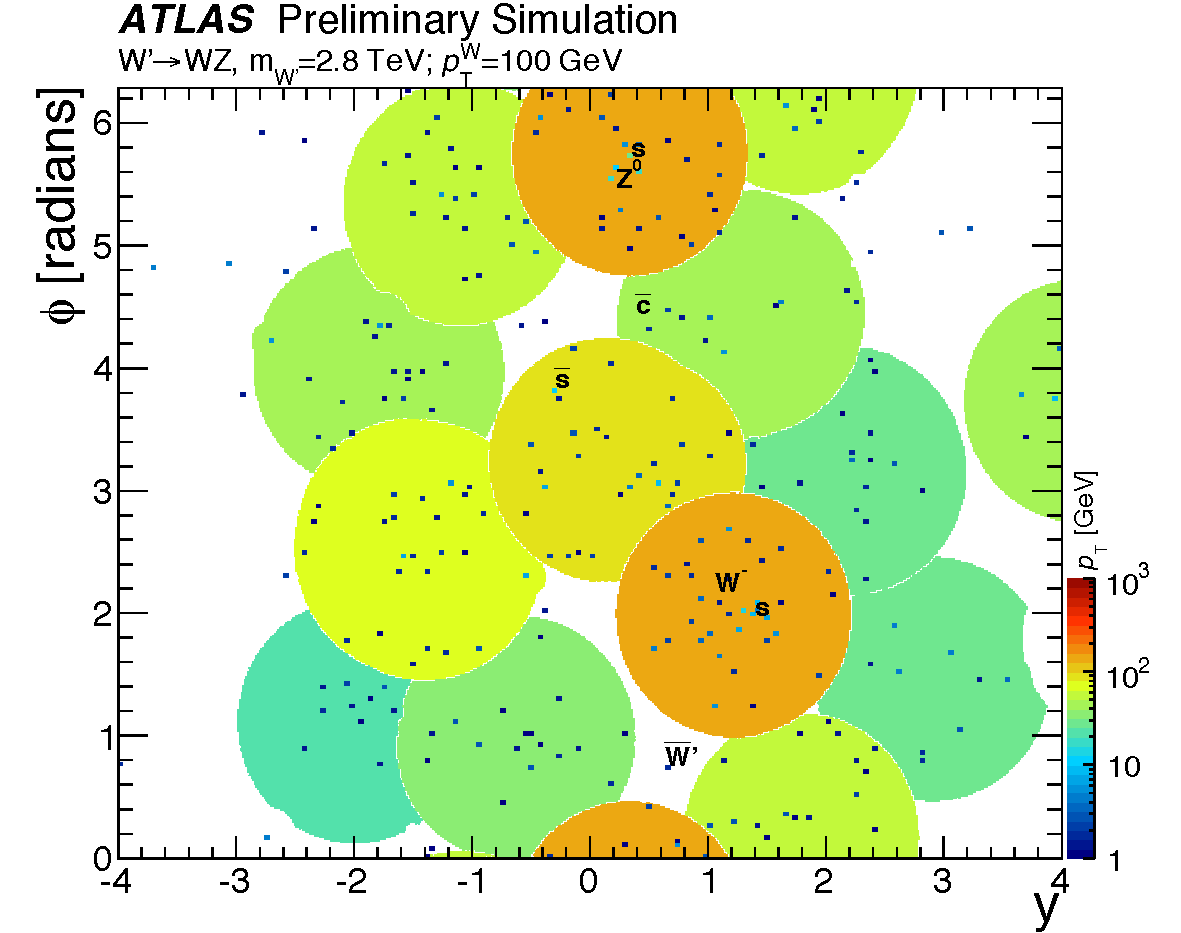
\includegraphics[width=0.7\textwidth]{akt.pdf}
\label{fig:jets:akt}
\caption{An example of a simulated ATLAS $W'\rightarrow WZ\rightarrow qqqq$ event, clustered with the \antikt algorithm with $R=1.0$.}
\end{figure}

%%%%%%%%%%%%%%%% 

Because the \antikt algorithm now provided a fast implementation and ``well behaved'' behavior, the LHC experiments quickly adopted it for use (though the Tevatron remained attached to cone algorithms for compatibility reasons). Typical $R$ parameters for ATLAS are $R=0.4$ and $R=0.6$: these sizes are large enough to capture the bulk of the radiation from a typical parton shower while minimizing contamination from overlapping partons and underlying event.


Does this mean that \kt and \CA algorithms have no use at the LHC? On the contrary, there are situations where they provide more information than \antikt. For example, the branching structure (or the clustering history) in these algorithms is considered meaningful: as softer particles are clustered first, it naively resembles the tree-structure of QCD showering, with each new pairing ``reversing'' a potential QCD splitting (as Figure~\ref{fig:jets:showering} demonstrates schematically). Similar information with the \antikt algorithm is hard to come by: the clustering history reveals only the seed-type interaction of a harder particles tending to attract others to them. Thus, analyses that seek to understand the structure of energy flow are more likely to use the \kt or \CA algorithms.

%%%%%%%%%%%%%%%%

\begin{figure}
\centering
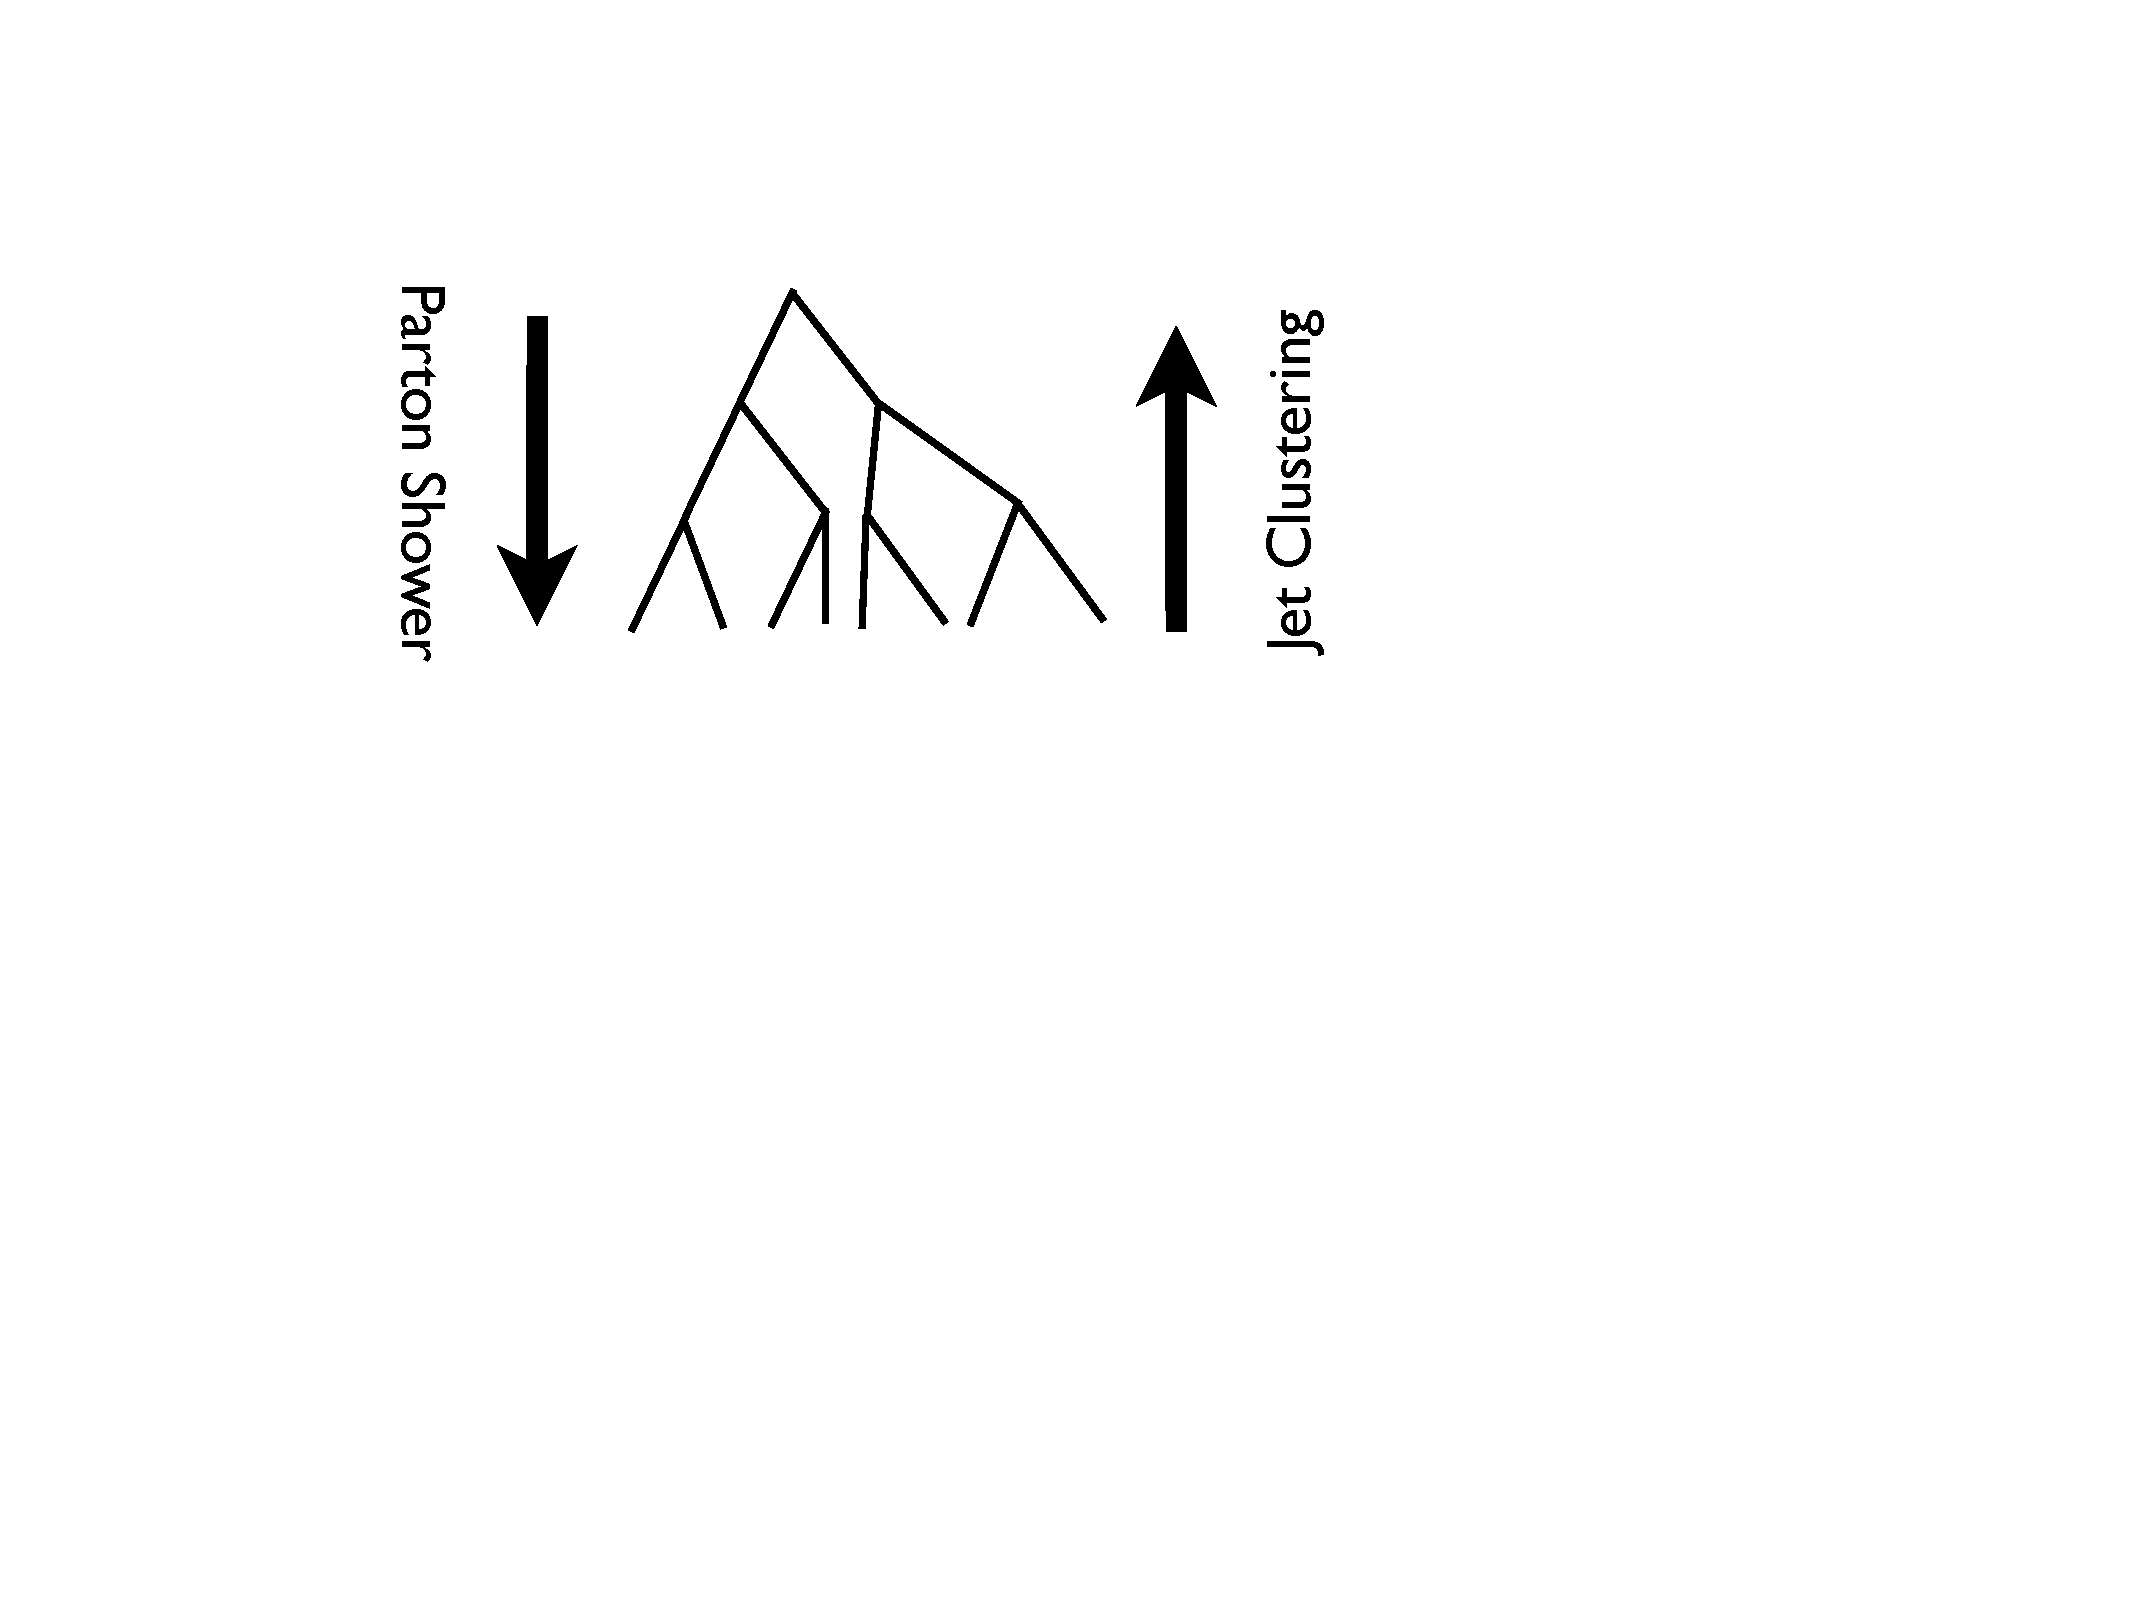
\includegraphics[width=0.7\textwidth]{showering.pdf}
\label{fig:jets:showering}
\caption{A schematic showing the type of structure the \kt algorithm is expected to reveal due to its \pt ordered clustering.}
\end{figure}

%%%%%%%%%%%%%%%% 


\section{Jet Substructure: Going Deeper}

This idea of looking at the clustering history or energy structure  of a jet is actually quite different from anything else we have discussed so far. Most analyses, at the Tevatron especially but even now at the LHC, simply consider a jet as a 4-vector corresponding to some parton\footnote{And even then this overstates the amount of information used--- most analyses essentially ignore the jet mass, reducing it to a 3-vector!}. This construction of a single 4-vector was indeed the whole point of the jet algorithm, so it is in some sense a triumph to have reduced the complexity of thousands of particles into a handful of well defined jets. But the sheer scale of this reduction raises the question: what information have we removed? Can we aid our understanding of the event by using some additional pieces?

This question becomes particularly interesting in the era of \textit{boosted physics} at the LHC. The unprecedented collision energy of the LHC mean that $W$ and $Z$ bosons, for example, can be produced not just essentially at rest, as was the case at LEP and the Tevatron, but with substantial momentum. This means that their decay products will often be collimated, as Figure~\ref{fig:jets:boost} shows. The angular separation, in fact, goes as approximately \editnote{Derive this}
%
\begin{equation}
R = \frac{2 m}{\pt}.
\end{equation}
%
Generally, this means that the decay products $W$ bosons with $\pt > 200$~GeV, or top quarks with $\pt > 350$~GeV when using two separate $R=0.4$ jets. This potential for overlap motivates a new approach, where one \textit{large $R$} jet is used to measure the hadronically decaying particle. The mass and \textit{substructure} of this jet can then be used to distinguish it from backgrounds~\cite{Jetography}.

%%%%%%%%%%%%%%%%

\begin{figure}
\centering
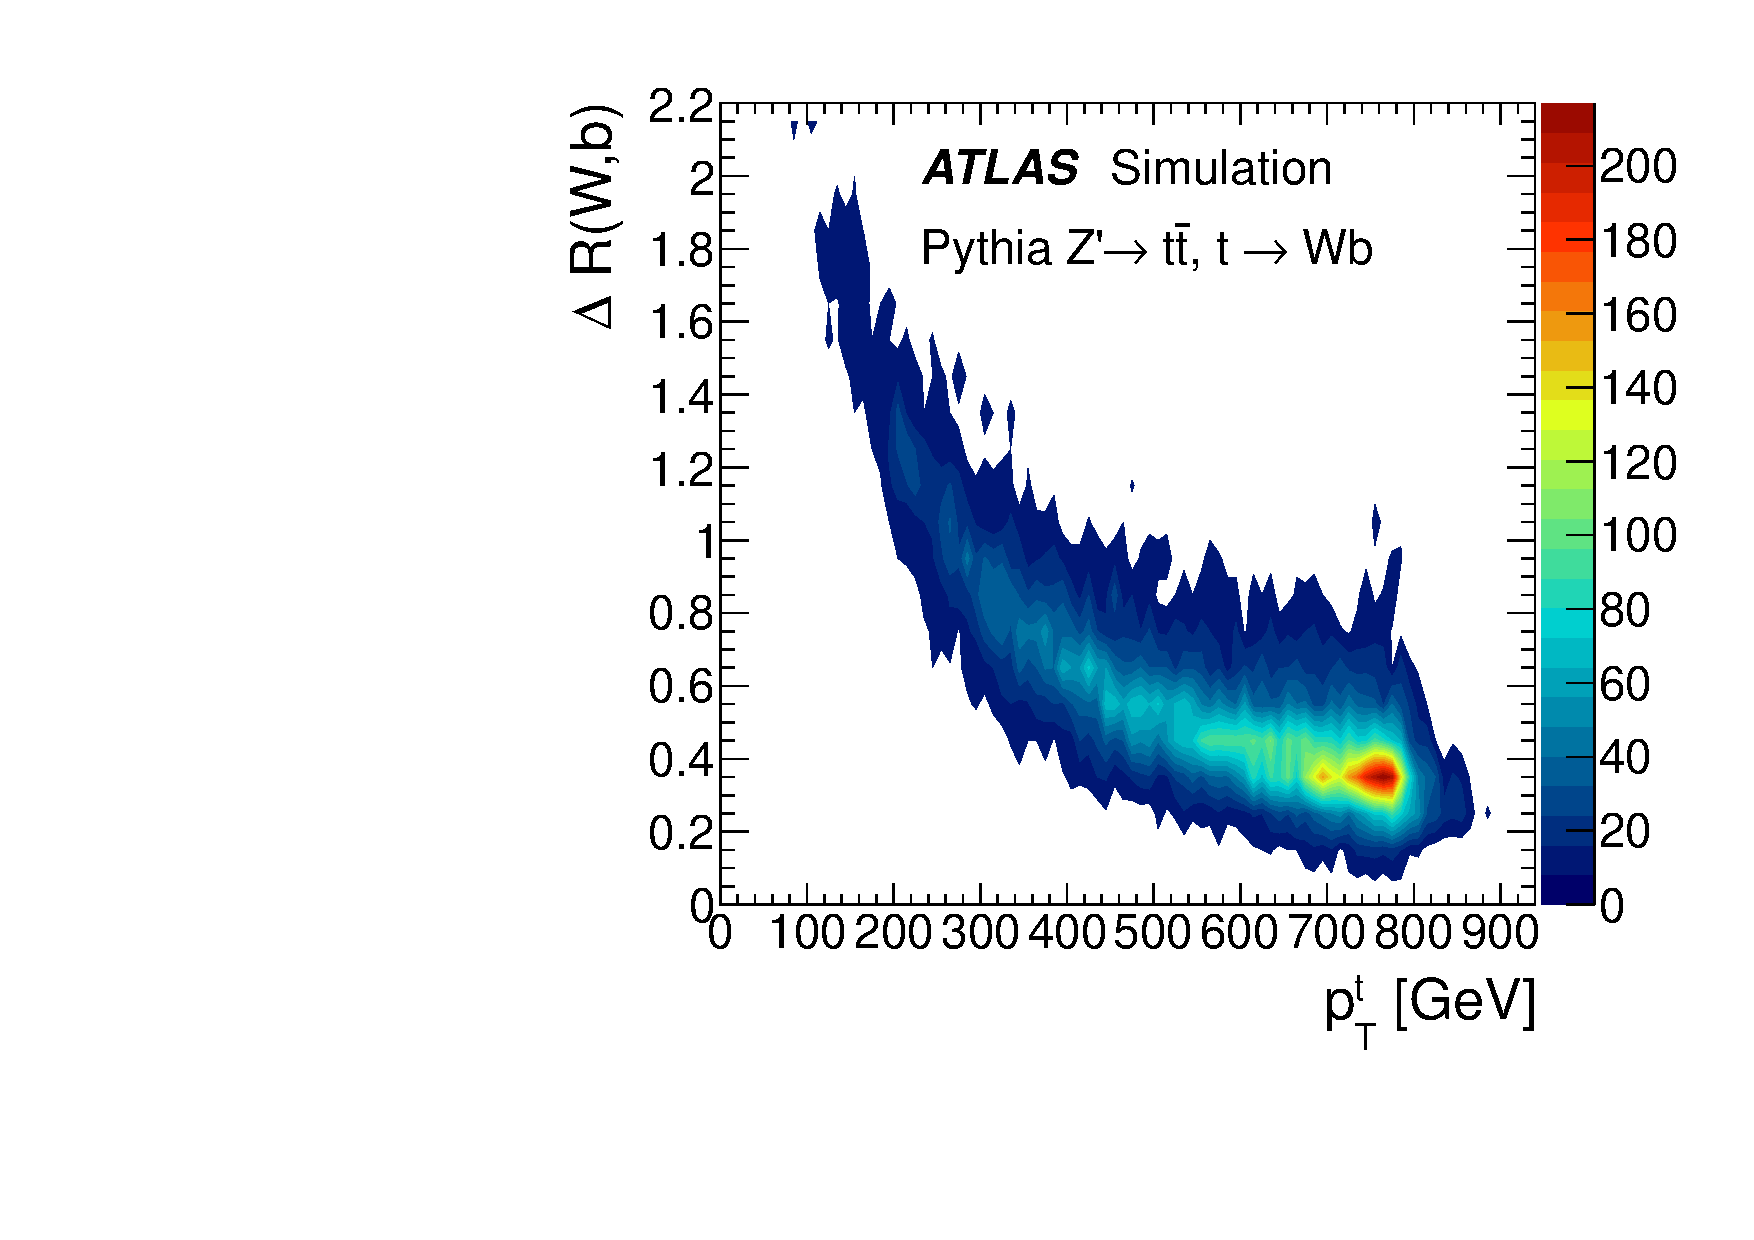
\includegraphics[width=0.45\textwidth]{boost_top.pdf}
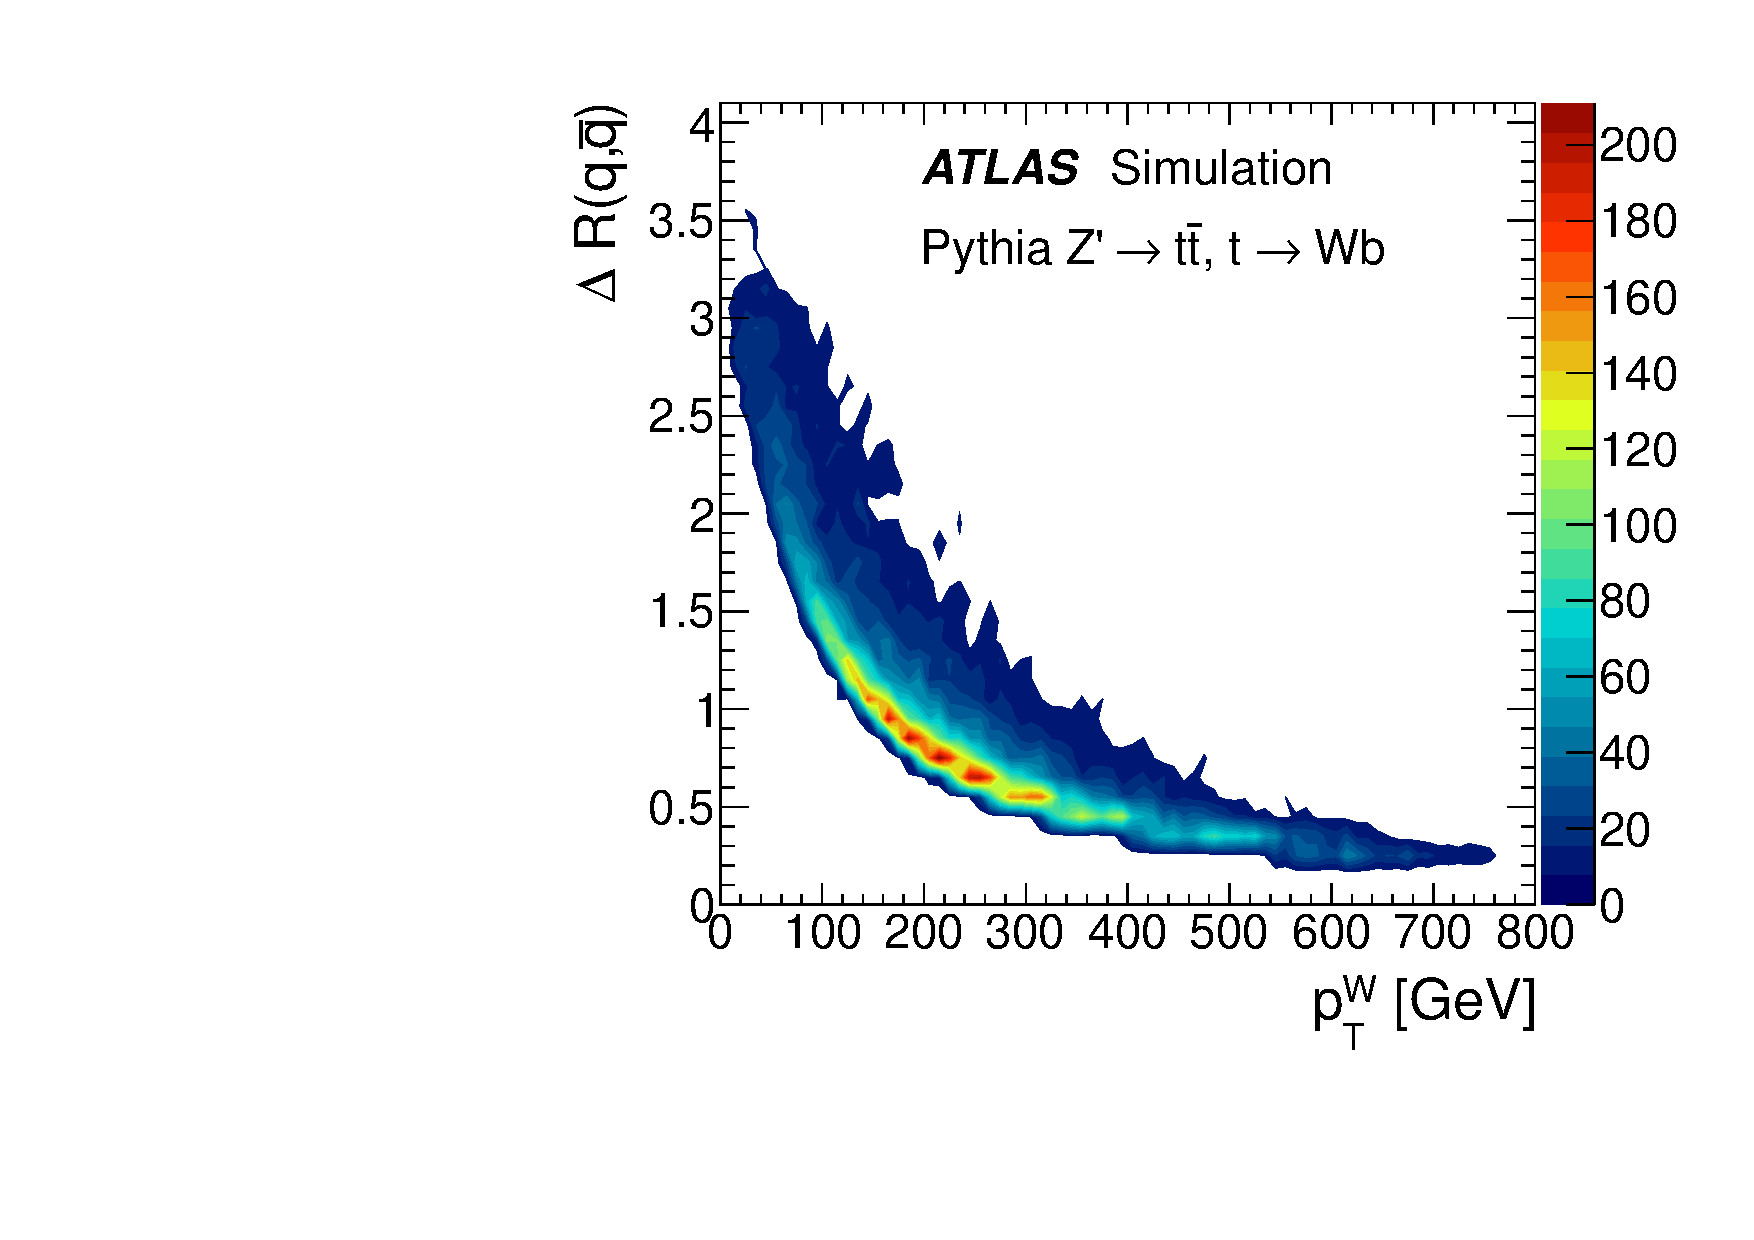
\includegraphics[width=0.45\textwidth]{boost_w.pdf}
\label{fig:jets:boost}
\caption{The angular separation $\Delta R$ between decay products in a $Z'\rightarrow t\bar{t}$ event as a function of the top \pt, and in a $W'\rightarrow WZ$ event as a function of boson \pt.}
\end{figure}

%%%%%%%%%%%%%%%% 

% 2m /pt

%BDRS

While earlier studies had suggested similar ideas~\editnote{cite!}, the seminal ``BDRS'' paper inspired a new flurry of activity by suggesting that it was possible to observe the decay boosted Higgs boson to $b\bar{b}$ by reconstructed  it within a single jet and tagging it with substructure \cite{BDRS}. Hadronic decays of the Higgs had previously been considered inaccessible at the LHC, so the suggestion that a new reconstruction technique might be able to measure it proved very exciting. At the heart of the idea is that the mass of the jet should correspond roughly to the Higgs mass, while the mass of jets from QCD backgrounds should be significantly lower. Moreover, the several-prong structure of a Higgs decay should be fairly unique compared to dominantly single-prong QCD backgrounds.

Since then, similar techniques have been extended to the reconstruction of top quarks, electroweak bosons, supersymmetric gluinos and stop quarks, and more~\editnote{Cite}. These analyses generally share several characteristics:
%
\begin{itemize}
\item Aim to reconstruct the boosted object with a single, \largeR jet, typically $R=1.0$ or $R=1.2$
\item \textit{Groom} the jet to remove the contamination of pileup and underlying event 
\item \textit{Tag} the jet by analyzing its structure to determine whether it is compatible with the boosted object hypothesis
\end{itemize}
%
While there are many different ways of approaching these points, the unifying theme is treating the jet as more than a 4-vector. 

\subsection{Grooming}
\label{chapter:jets-and-substructure:grooming}

One potential for concern when reconstructing jets with \largeR is contamination: a large size is used to capture all the collimated decay products within a single jet, but also opens up the jet to extra unwanted radiation from beam remenants and overlapping proton-proton collisions. This extra radiation, even if it is soft and does not affect the energy of the jet very much, can still have a large impact on the mass of a jet: the mass of a jet is determined by the angular splittings between its consituents, and even soft radiation at a wide angle can increase the mass dramatically.

Jet grooming is the strategy of modifying jet algorithms to remove these effects. Typically a normal jet algorithm is run to create a parent jet, and then a subsequent processing reconsiders the jet and removes portions that are considered unnecessary. A wide range of algorithms exist for this modification step--- filtering, pruning, and trimming are the most common~\editnote{Cite}. The most commonly used of these in ATLAS is trimming, which procedes as follows:
%
\begin{enumerate}
\item Start with a clustered \largeR jet, typically \antikt\ with R=1.0
\item Choose a \textit{subjet} algorithm and size, typically $\Rsub = 0.3$ and \kt
\item Remove all subjets with \pt smaller than some fraction \fcut of the original jet's \pt, typically $\fcut  = 5\%$
\item The 4-vector sum of the remaining subjets is the trimmed jets
\end{enumerate}
%
This algorithm explicitly targets the soft radiation--- typically at wide angle--- which can raise the mass of QCD jets and help them ``fake'' boosted objects. Figure~\ref{fig:jets:trimmed} shows again the same event we have been examining in previous sections, but this time with the trimming algorithm applied. The empty areas correspond to parts of the jet that have been removed; the various grayscale remaining areas indicate the surviving subjets and their relative \pt fraction. 


%%%%%%%%%%%%%%%%

\begin{figure}
\centering
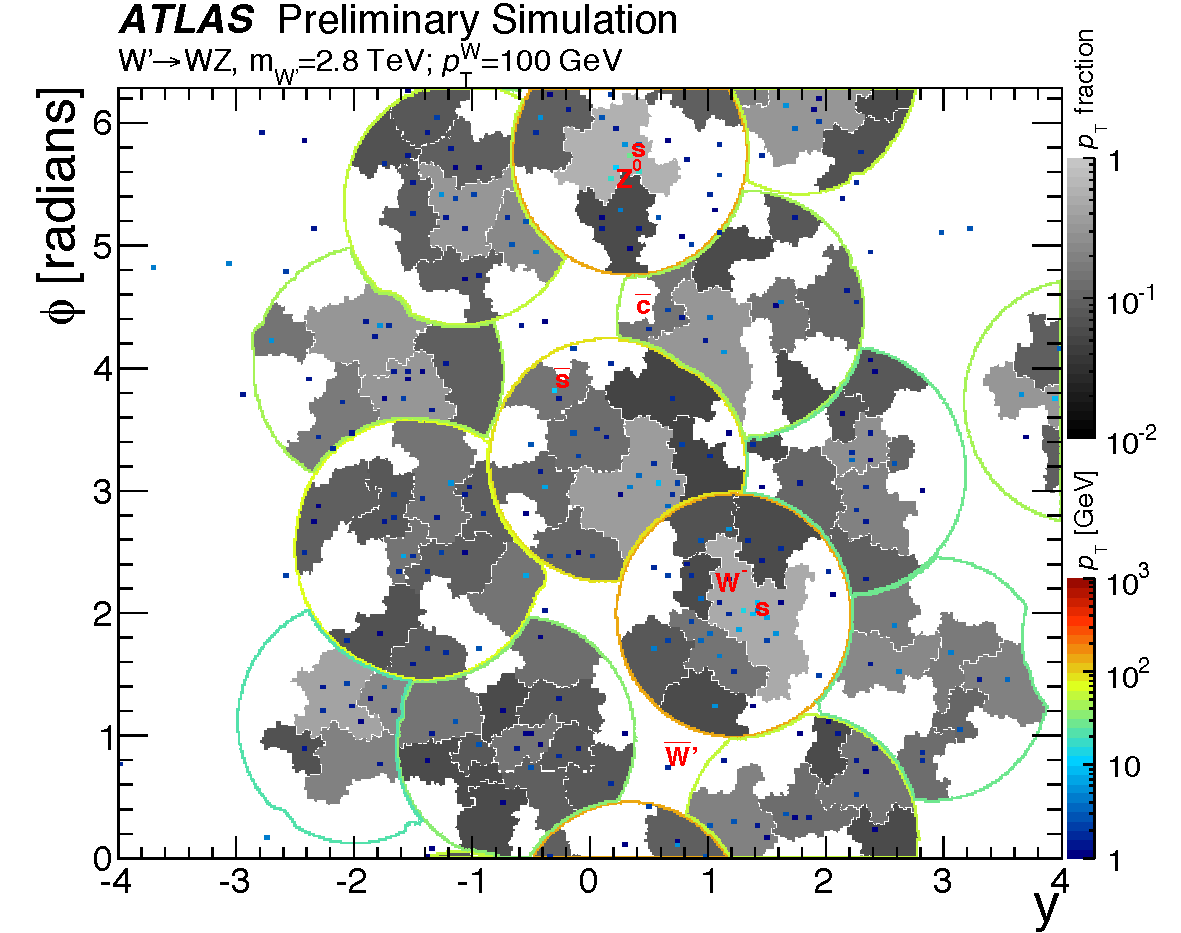
\includegraphics[width=0.7\textwidth]{trimmed}
\label{fig:jets:trimmed}
\caption{A event display, identical to Figure~\ref{fig:jets:akt} except after trimming with $\Rsub = 0.3$ and $\fcut = 5\%$ is applied.}
\end{figure}

%%%%%%%%%%%%%%%% 

How well does trimming work in practice? Figure~\ref{fig:jets:z_trimming} shows the reconstructed mass of a boosted $Z\rightarrow qq$ decay, with the red lines showing the signal and the black a QCD multi-jet background. The solid lines are the masses with just an \antikt\ $R=1.0$ algorithm; the dashed lines are after trimming. The improvement in discrimination power is dramatic, and demonstrates why trimming is an integral part of ATLAS's boosted object studies.


%%%%%%%%%%%%%%%%

\begin{figure}
\centering
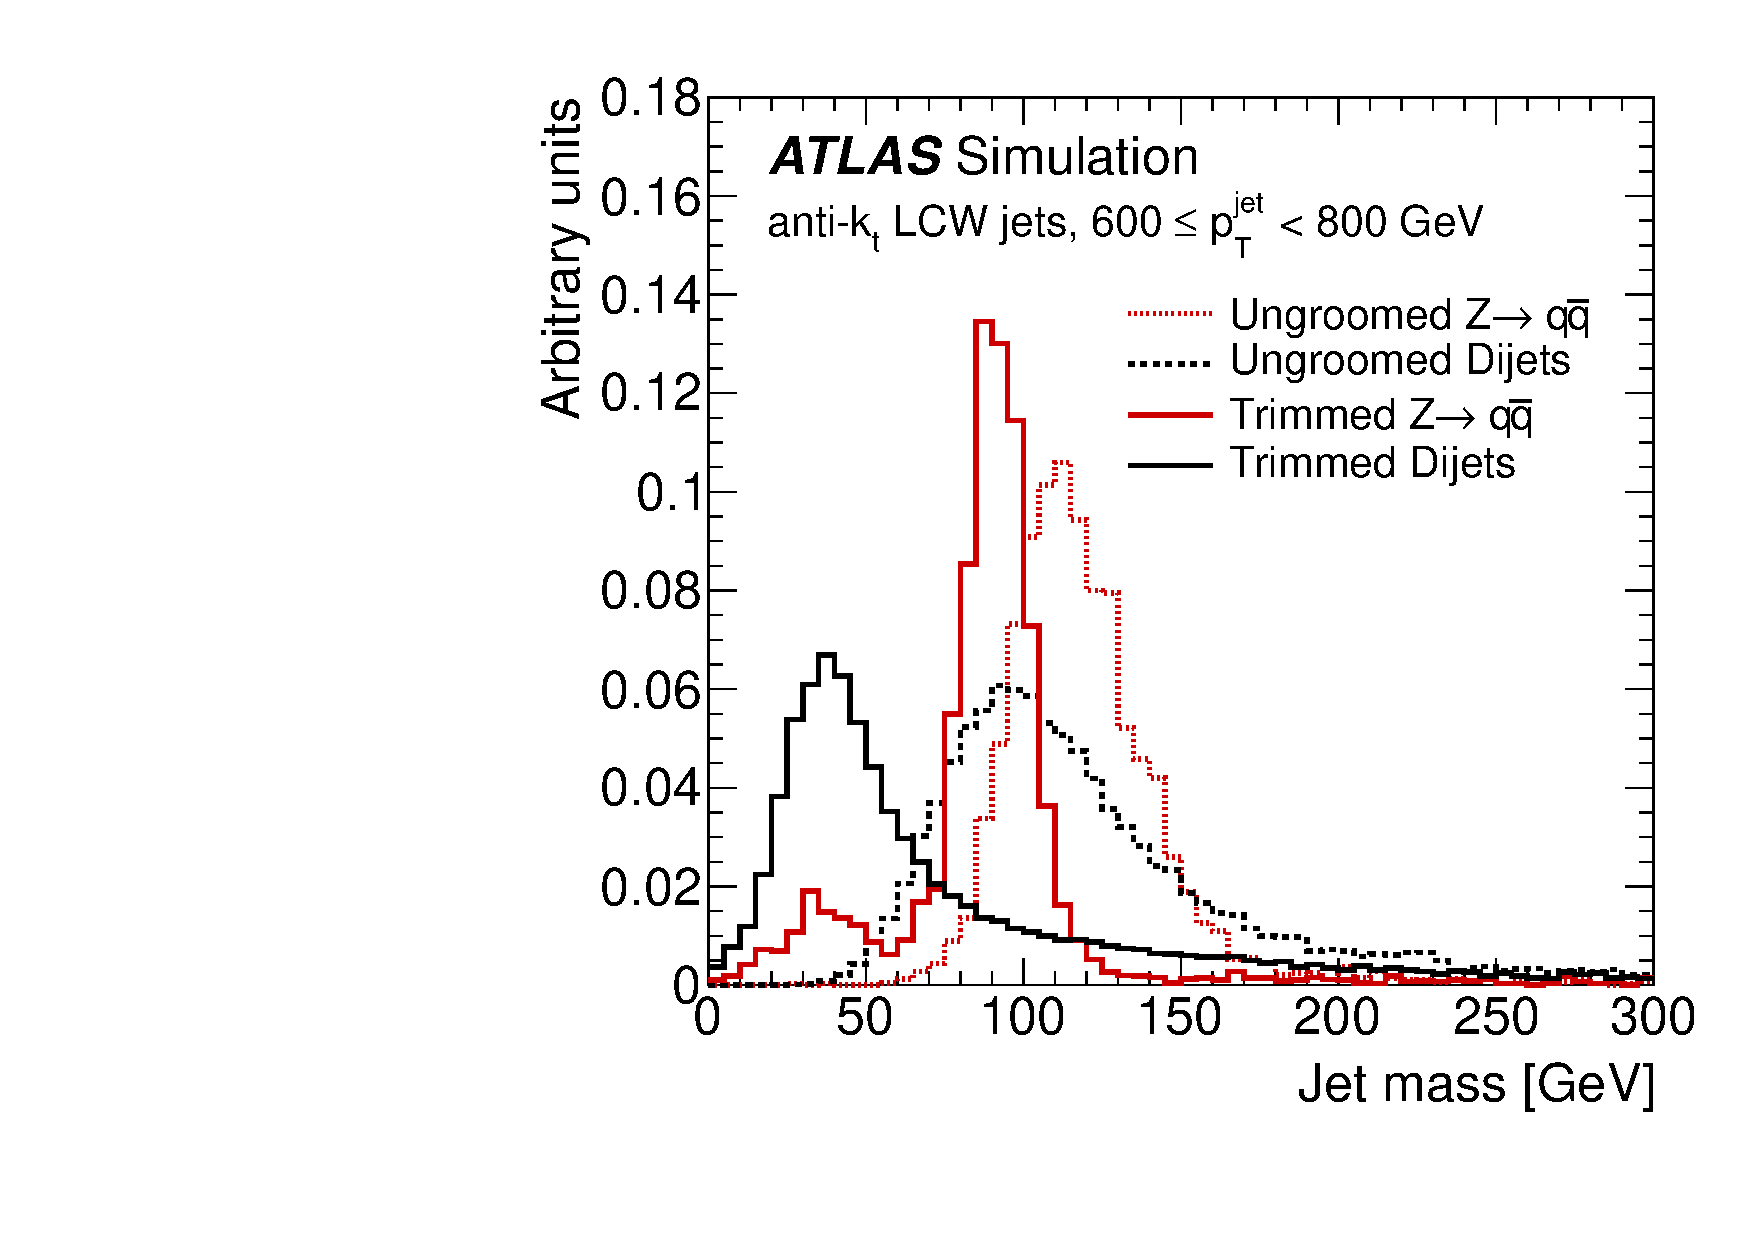
\includegraphics[width=0.7\textwidth]{z_trimming}
\label{fig:jets:z_trimming}
\caption{A plot of jet masses for a signal $Z\rightarrow qq$ decay and QCD multijet backgrounds in red and black respectively. The solid lines indicate the mass before trimming, and the dashed lines after trimming.}
\end{figure}

%%%%%%%%%%%%%%%% 


\subsection{Tagging}

The second part of the BDRS program was the identification of substructure in the event: QCD jets can fake a jet mass requirement due to the overwhelming size of the backgrounds, but additional criteria on the shape could help remove even more background. The BDRS approach implemented cuts at the grooming level to reject unbalanced jets and other characteristics common to backgrounds~\cite{BDRS}. As with grooming techniques, a whole library of tools have emerged to discriminate between various signals and QCD multi-jet backgrounds. 

One powerful technique which will come up again in Chapter~\ref{chapter:search} is referred to as $n$-subjettiness~\cite{nsub}. $N$-subjettiness aims to measure how compatible a given jet is with an $n$-subjet hypothesis: by quantifying this as a real number, instead of an integer, a wider range of values without sharp cuts are able to be studied. Denoted $\tau_N$, it is calculated as follows:
%
\begin{enumerate}
\item Identify $N$ axes in some fashion; often, the exclusive \kt\ algorithm is run to create $N$ subjets and those axes are used\footnote{The exclusive \kt\ algorithm is identical to the one already introduced, but with a different stopping condition: $R$ is set arbitrarily large so that it will never stop the clustering, and instead the procedure stops when $N$ jets are identified.}.
\item Loop over the constituents $k$ of the jet and calculate:
\begin{equation}
\tau_N = \frac{\sum_k \pT^k \min(\Delta R(N,k))}{\sum_k \pT^k R}
\end{equation}
where $R$ is the radius of the jet, and the minimization is performed over all axes defined in step 1.
\end{enumerate}
%
What is this variable actually doing? It calculates the distance to the closest available axis to each particle. If the particles of the jet were entirely lined up on the axes, this value would be 0. In principle, then a low value indicates a strong compatibility with an $N$-subjet hypothesis. In practice, it is also possible that a low value corresponds to compatibility with an $N-x$-subjet hypothesis: they could all be lined up along just one of the axes, for example. This motivates the use of n-subjettiness \textit{ratios}: $\tau_{MN} = \tau_M / \tau_N$, with $M > N$, which normalize away this lower-order agreement, if it exists. Figure~\ref{fig:jets:nsub} demonstrates the discrimination of the variable: the QCD background tends to have a higher value than the signal in both 3-body signal and 2-body signal decays. Figure~\ref{fig:jets:top_tagging} shows a comparison of the performance of various top-taggers by plotting the efficiency of selecting top quarks on the $x$-axis and the inverse efficiency for selecting multi-jet background events. $N$-subjettiness selections tend to be strongest at high signal efficiency, while other techniques are able to achieve better background rejection at lower signal efficiency.

%%%%%%%%%%%%%%%%

\begin{figure}
\centering
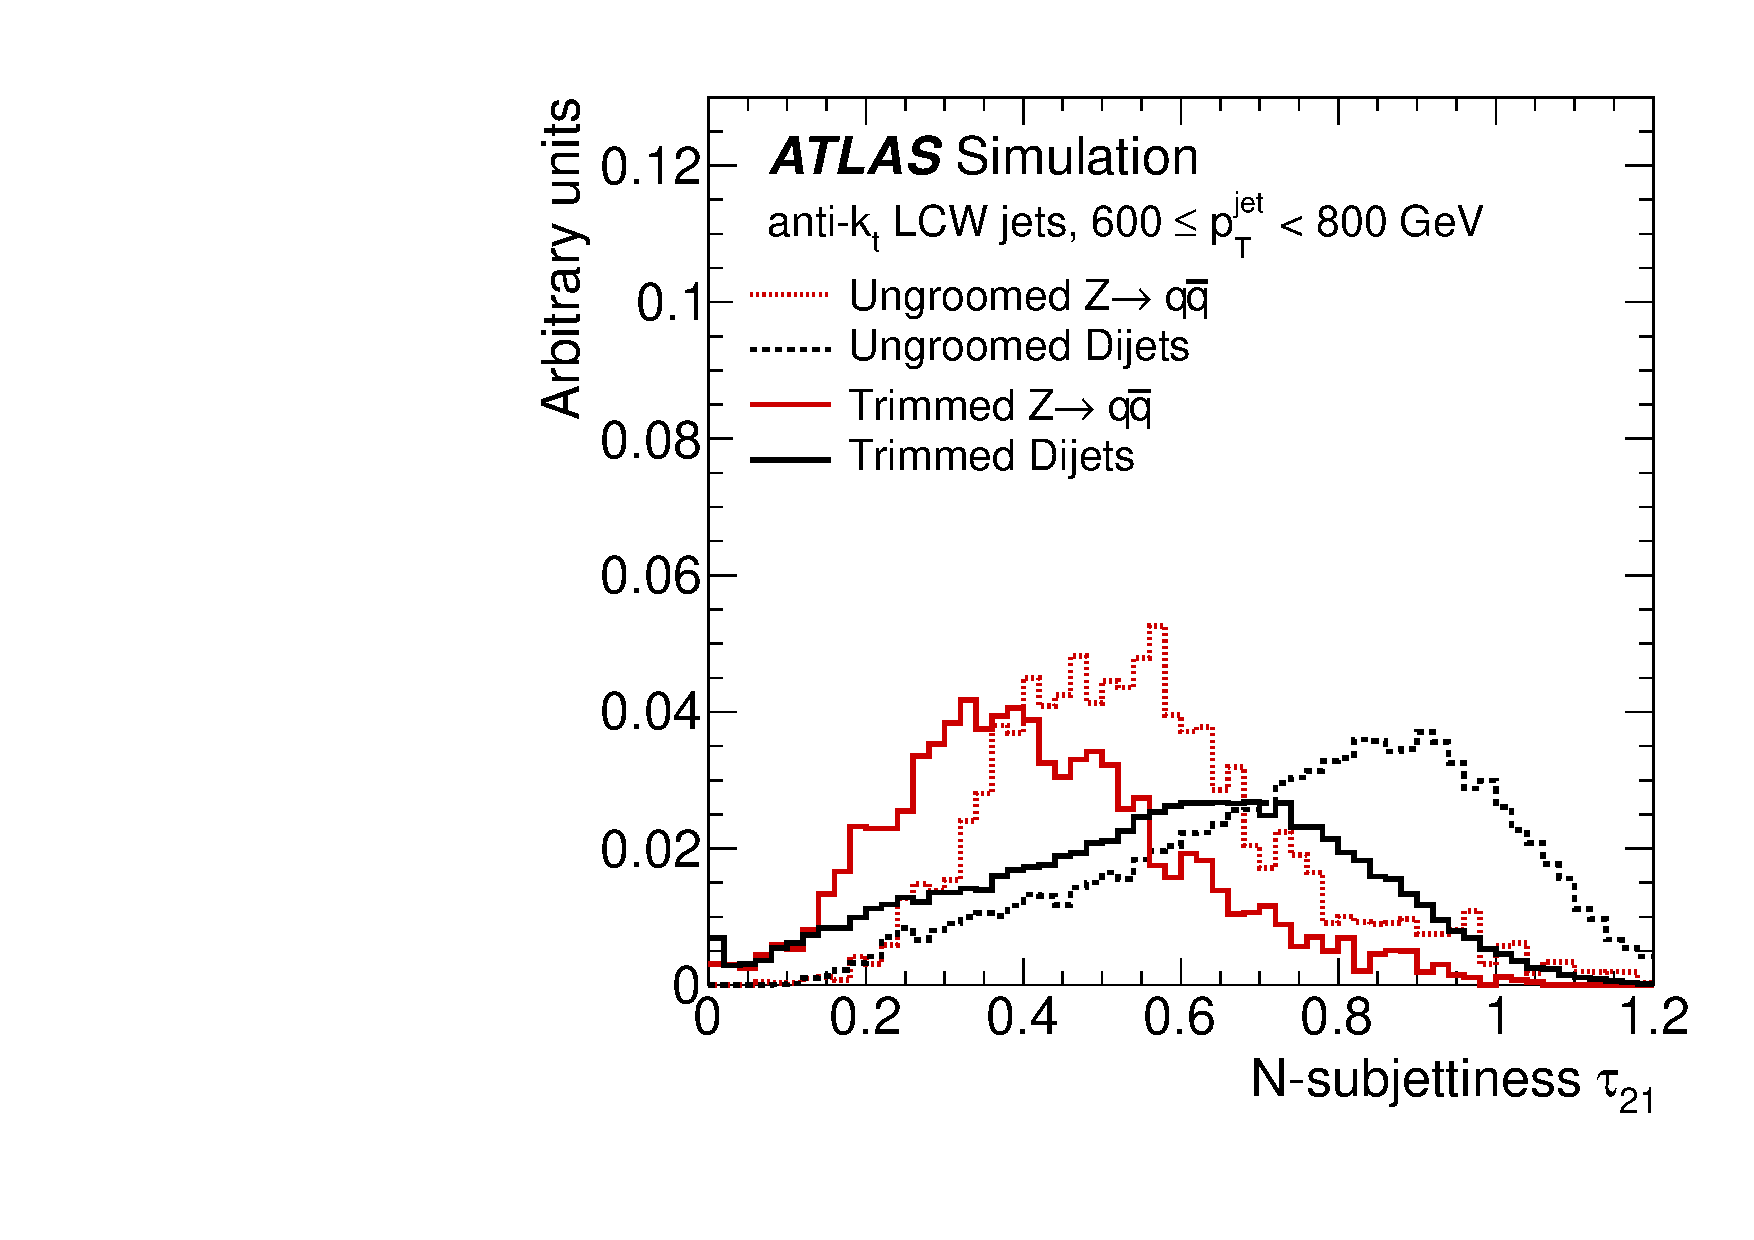
\includegraphics[width=0.45\textwidth]{nsub_21.pdf}
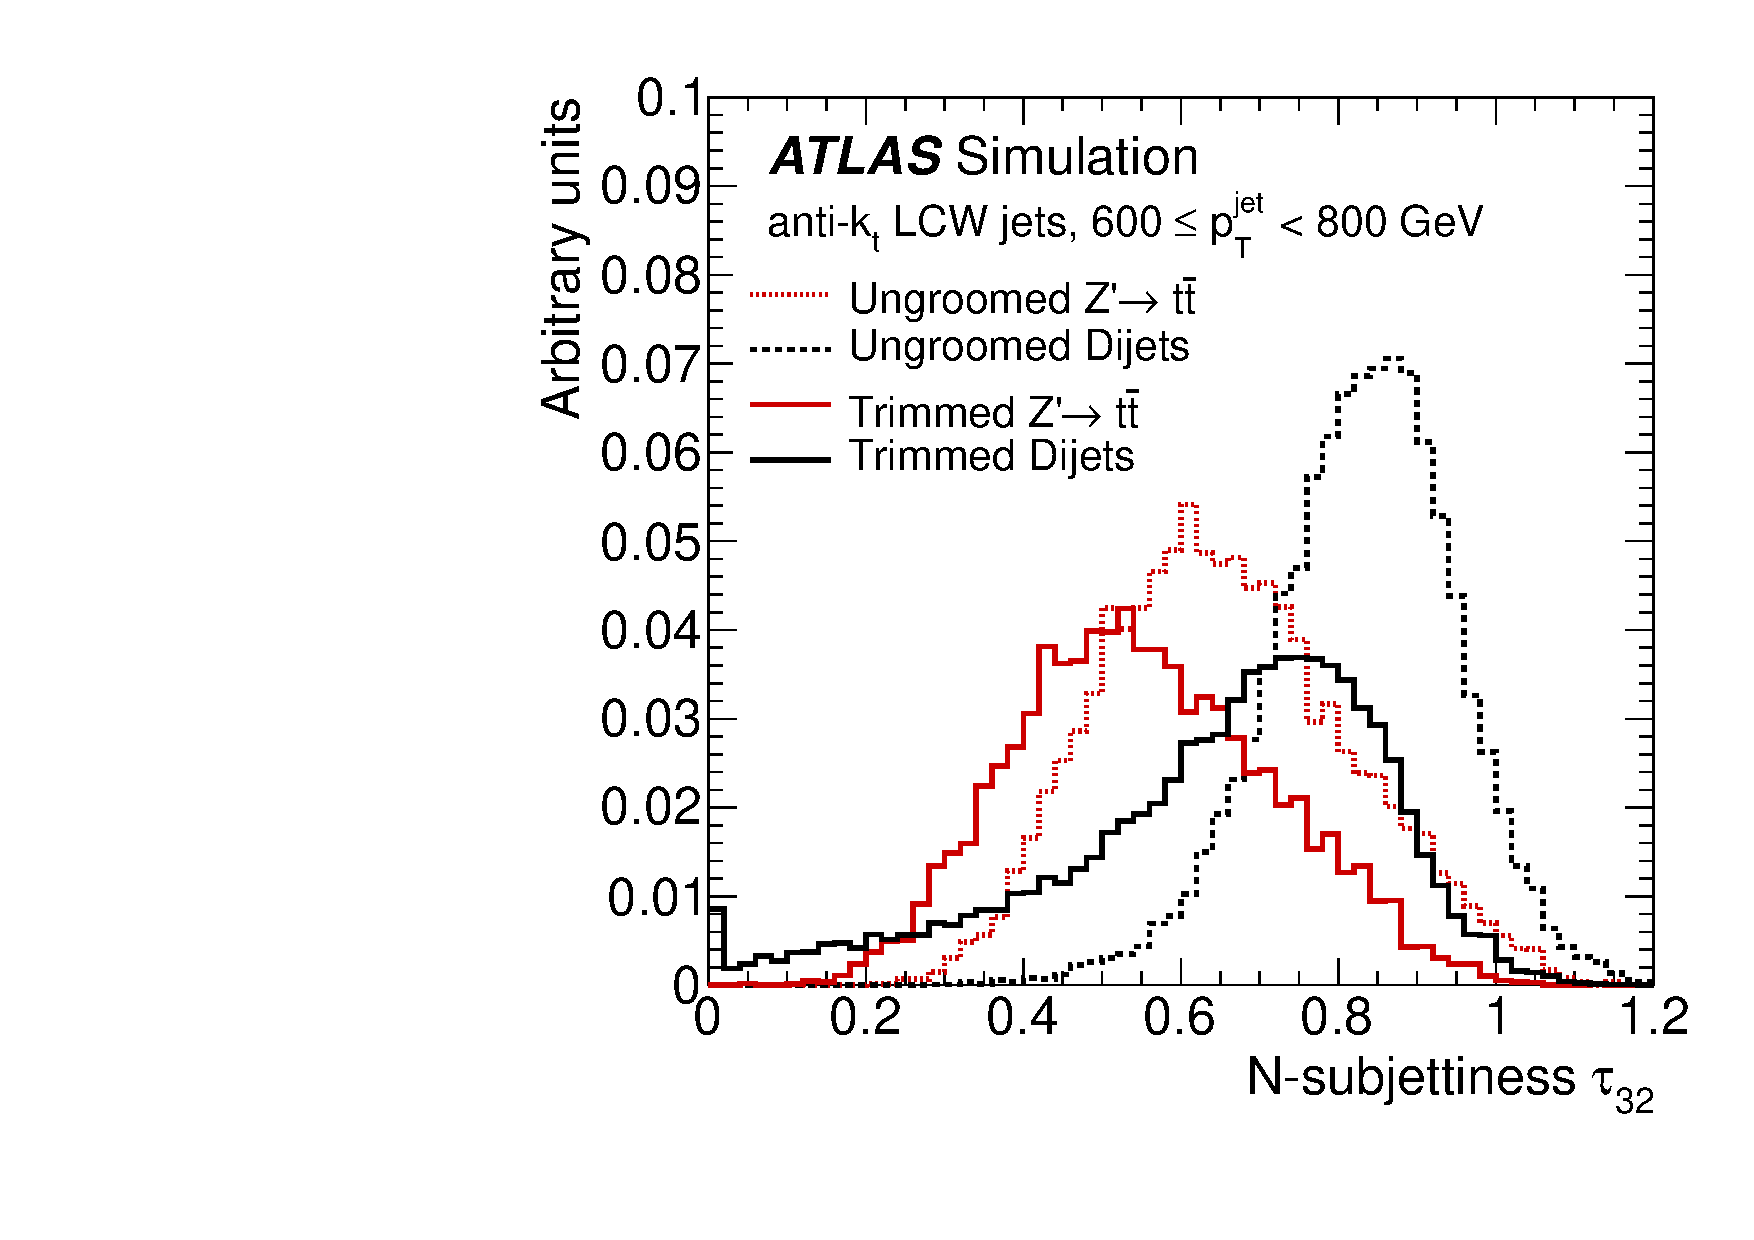
\includegraphics[width=0.45\textwidth]{nsub_32.pdf}
\label{fig:jets:nsub}
\caption{$n$-subjettiness ratios $\tau_{21}$ and $\tau_{32}$ for signal events (hadronically decaying $Z$ bosons and top quarks, respectively) compared to QCD multi-jet backgrounds. The solid lines indicate the value before trimming, and the dashed after trimming.}
\end{figure}

%%%%%%%%%%%%%%%% 


%%%%%%%%%%%%%%%%

\begin{figure}
\centering
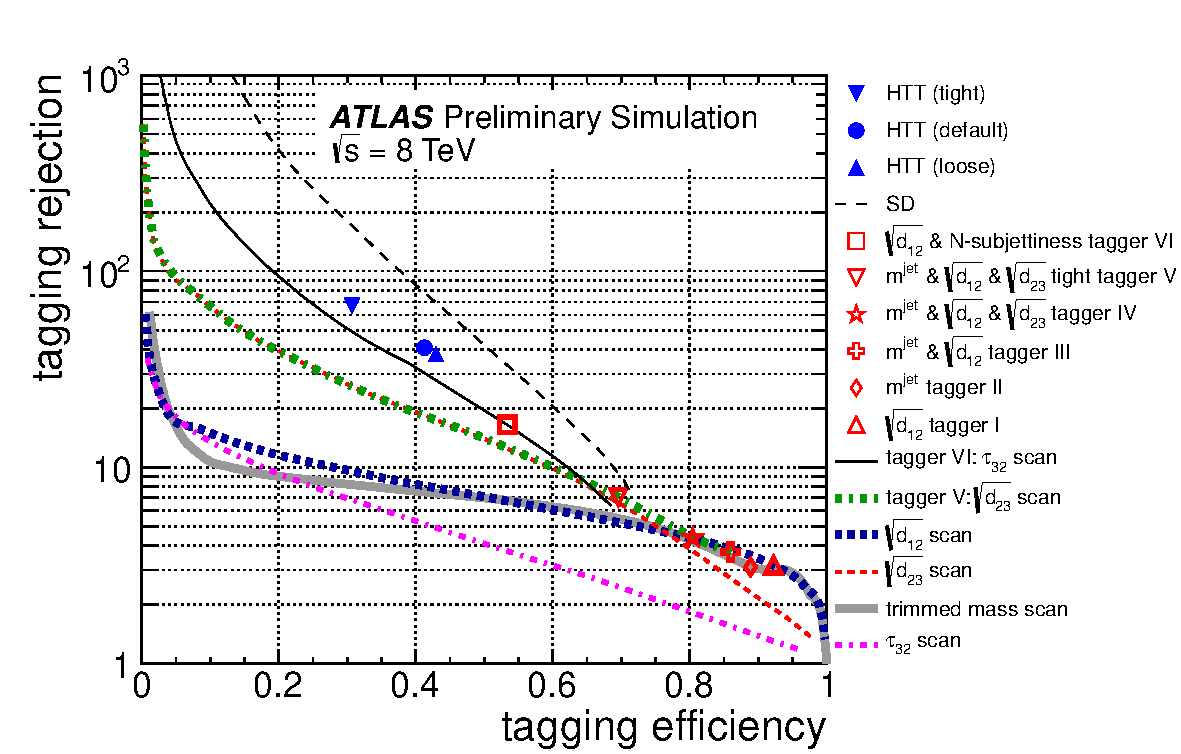
\includegraphics[width=0.7\textwidth]{top_tagging}
\label{fig:jets:top_tagging}
\caption{A comparison in signal (top quarks) efficiency and background (QCD multi-jet) rejection for various top-tagging algorithms.}
\end{figure}

%%%%%%%%%%%%%%%% 



%\section{Calculations with Jets}

Many different analyses in ATLAS, most of them searches for new physics in various high mass channels, have utilized these substruture techniques. Hadronic decays of top quarks and bosons often have the dominant branching fractions, and high mass systems create strongly collimated signals, making these techniques the bedrock of a new type of analysis. \editnote{cite this}

\section{Conclusions}

So, having gone through an entire chapter--- what is a jet?

Having explored so many different possibilities, it should be clear that there is no easy answer: instead, we should always be aware that a jet is an \textit{algorithm} and that it is a \textit{choice}. As physicists, we choose the parameters of our algorithm and the type of reconstruction we perform; depending on what we are doing, and what our detector is capable of, different algorithms are appropriate. Jets always correspond to some spray of particles initiated by a QCD parton, but the details of hadron-hadron interactions or boosted object decays can make the situation much more complicated.

The key innovation over the career this PhD corresponds to is the shift towards recognizing jets as more than 4-vectors. Unprecedented detectors with granularity much improved over previous designs, as well as improved theoretical understanding and development, has enabled us to pick out information from inside jets that we otherwise would have left behind. This enables not only new types of searches for new physics with boosted objects, as previously alluded to, but also entirely new measurements of properties of the Standard Model: these ideas are at the heart of the experimental analyses of this thesis.

